\documentclass{article}

\usepackage[utf8]{inputenc}
%\usepackage{url}
\usepackage[pdftex]{graphicx}
\usepackage{xspace}
\usepackage{geometry}
\usepackage{pstricks}
\usepackage{color}

\newcommand{\softName}{{\em LIPN UIMA Platform}\xspace}
\newcommand{\archiveName}{lipn-uima-core.tgz}
%\newcommand{\archiveName}{lipn-uima-core-0.1.3.tgz}
\newcommand{\urlVersionStable}{http://www-lipn.univ-paris13.fr/~moreau/uima/\archiveName}
\newcommand{\versionSoft}{0.1.*}
\newcommand{\dateLastUpdate}{May 2011}

%_____ Pour la génération des hyperliens & URL
\usepackage[colorlinks=true,linkcolor=black,urlcolor=black,citecolor=black]{hyperref} %,hyperfootnotes=false


\author{Erwan Moreau\\ {\tt Erwan.Moreau@lipn.univ-paris13.fr}}
\title{{\sf Technical Report \\ \ \\ \softName \versionSoft\\ User/developer guide }}
\date{October 2010 \\ {\small last update: \dateLastUpdate}}


% page layout
\geometry{hmargin=2cm, vmargin=2.5cm}
\addtolength{\parskip}{0.75\baselineskip}
\setlength\parindent{0pt}
\newenvironment{xenumerate}{
\begin{enumerate}
  \setlength{\itemsep}{.3\baselineskip}
  \setlength{\topsep}{0pt}
  \setlength{\parskip}{0pt}
  \setlength{\parsep}{0pt}
}{\end{enumerate}}
\newenvironment{xitemize}{
\begin{itemize}
  \setlength{\itemsep}{.3\baselineskip}
  \setlength{\topsep}{0pt}
  \setlength{\parskip}{0pt}
  \setlength{\parsep}{0pt}
}{\end{itemize}}



\newcommand{\todo}[1]{{\large \sf [TODO #1]}}
\newcommand{\rien}[1]{}


\newcommand{\packname}{fr.lipn.nlptools}
\newcommand{\utilsPackname}{\packname.utils}
\newcommand{\uimaPackname}{\packname.uima}
\newcommand{\uimaModule}{{\em lipn-uima-core}\xspace}
\newcommand{\utilsModule}{{\em lipn-nlptools-utils}\xspace}
\newcommand{\glossEntry}[2]{{\bf #1} #2}

\begin{document}

\maketitle

\tableofcontents

\newpage


\section{Introduction}

This document describes the ``\softName'' software, developed in 2010 by the author at LIPN\footnote{This work was funded by OSEO the Quaero project. The preliminary steps of this work were implemented by Sondes Bannour. The author also thanks Fabien Poulard, PhD student at LINA, who helped him a lot to understand UIMA mechanics during this work.}. This software mainly consists in a UIMA-based evolutive platform devoted to corpora annotation. It is divided into two modules (\uimaModule and \utilsModule) and is distributed as an archive containing a environment providing a few tools (scripts, CPE descriptors, examples etc.). Currently the software is located\footnote{If the link does not exist anymore, please contact the author.} at:

\begin{center}
\url{\urlVersionStable}
\end{center}


\label{partModulesDescription}
{\em Remark.} Two modules are provided: UIMA-dependent packages (annotators etc.) belong to \uimaModule, whereas all other packages belong to \utilsModule\footnote{Actually the latter still depends on the {\em uima-core} package, but only because the UIMA {\tt Logger} class is used (this technical point is not significative).}. The latter is contained in the former archive as a JAR package, but can also be found as a standalone archive at the same address.



\subsection{Preamble: what this guide is (and is not)}


The \softName components are quite complex. This document is intended to help the user understand what are their goals, how they can be used, and the reasons of various design/implementation choices. It is mainly thought as a ``user guide'', not as an exhaustive documentation: for precise documentation on some class/method/parameter, {\bf please refer to the  Javadoc API}. This document is {\bf neither a UIMA tutorial}: to obtain information about this framework please see the UIMA official site (see \ref{partUimaHelp}). It is rather intended to propose a global point of view on the \softName components, with explanations about how these components work together. It also details the conventions/guidelines which have been used, and that the user should preferably also follow when coding new components using/relating/belonging to \softName. Thus this guide is intended to different kind of readers/users:
\begin{xitemize}
\item If you\footnote{In these sentences ``you want to ...'' can be replaced with ``your PhD advisor asked you to ...'' if applicable.} only want to run the components from a Java program or from a command line, see \ref{partRunNoUima}.
\item If you only want to use the UIMA independent packages, see \ref{partUimaIndependentCode} and API.
\item  If you have at least basic knowledge about UIMA (main audience) and you want to be able to use the components in an unconstrained UIMA environment, you should preferably have a look at all sections, but you can esily skip details/implementation parts (in particular section \ref{partUimaIndependentCode}). Do not forget to read details about the annotators parameters in the descriptors files.
\item If you plan to develop new UIMA components using \softName ones the same applies, but you should probably skip less parts.
\item If you want to correct/improve the components that this document describes, I humbly suggest you read the whole guide (and I will probably hear about you sooner or later!)
\end{xitemize}

The structure of this document is perhaps a bit confused, because there are many ways to tackle UIMA software in general and this one in particular. This user guide should hopefully make clear most aspects of the components, but feel free to contact the author if you think something is wrong/missing/should be improved\footnote{The author also apologizes for the very poor English in this document, sorry!}. 
\smallskip

\subsection{Main objectives and content}

These software components were created in the following goals:
\begin{xitemize}
\item Update/improve existing software tools used at LIPN, mainly to make them more flexible (in the way to use them) and more robust. These tools are (more or less) those previously used in the {\em Ogmios/Alvis} platform (TreeTagger and YaTeA essentially). In this goal, tools are provided to use the corresponding components as ``black boxes'', allowing the user not to care about all the UIMA stuff.
\item Build the core of a UIMA platform devoted to LIPN research tasks (semantic annotation), in order to initiate a long-term approach towards a better organization of software developped in the lab. This is the main reason why UIMA has been chosen. In particular, we hope that future pieces of code will be more uniform, easier to combine with each other and also easier to maintain. Thus choices are made to make this platform as evolutive as possible.
\item Propose a new approach in the design of an NLP platform, with two main ideas:
\begin{xitemize}
\item Using a very {\bf generic {\em Type System}} (see \ref{partTypeSystem}) in order to promote the modularity of components in a processing pipe. Following UIMA's principles about making data transmission easier between different components not knowing about each other (or not much). 
\item Making possible and as convenient as possible the use of {\bf {\em concurrent annotations}} (see \ref{partConcurrentAnnot}). This point requires that components are designed in a way which makes it possible, and also suitable tools for a user.
\end{xitemize}
\end{xitemize}
\smallskip

As a side effect, this library also fulfill several other needs:
\begin{xitemize}
\item It provides tools for calling an {\em external program} (see \ref{partExternalProgram}) from Java in a quite robust, safe and convenient way. The library contains both  a UIMA independent component and a UIMA generic annotator (see \ref{partWrapper}).
\item It provides tools for re-aligning and/or converting structured data (mainly intended for NLP standard annotations format) in a uniform and modular way (see \ref{partAlign}). A UIMA independent package is provided, which can also easily be used inside UIMA.
\end{xitemize}



Most of the UIMA annotators provided in this library are {\bf wrappers} for previously existing tools. This choice is done for time and cost reasons: it is clearly more reasonable to use these existing annotation tools, among which some are LIPN expertise, rather than re-coding them from scratch in a ``pure'' UIMA environment. That is why these first components will actually be wrappers for what we call ``external programs'', in the sense that they run as a black box (in the UIMA platform viewpoint). This is clearly not the ideal situation: UIMA provides a very complete, convenient and safe environment for connecting annotators together in some complex system (error handling, logging, resources management, deployment, etc.), so calling external programs introduces a lot of possible flaws (portability problems, I/O errors, uncontrolled use of resources, concurrency errors, etc.). This a critical point because a complex task can involve quite a lot of different components, so it can be very vulnerable to any problem in the chain: clearly one does not want that the complete system fails because a single document makes a single component crash due for example to some minor charset encoding problem. 

Thus a large part of this work has been devoted to deal with these drawbacks with care. This is actually the reason why the code has been divided into two distinct modules: \uimaModule contains the real UIMA components, while \utilsModule is devoted to this kind of problems and consists in several utility packages which are (almost) UIMA independent (see \ref{partModulesDescription}).

One of the most important consequences about this recycling strategy is that the LIPN components are {\bf not portable} (at least they can not be considered portable). Due to the software used as external programs itself and/or the constraints to use it from inside the platform, all wrapper components are Linux (or Unix-like) only! The following (main) components are provided (most of them handle only English and/or French as language):

\begin{xitemize}
\item The {\bf TagEN} named entities recognizer (for French and English), created a few years ago at LIPN by Thierry Poibeau and Jean-François Berroyer. An updated version has been integrated to the platform. Warning: resources used by this tagger are a bit old.
\item The {\bf TreeTagger} Part-of-speech tagger\footnote{There is also a UIMA TreeTagger wrapper proposed by the LINA: \url{http://www.lina.univ-nantes.fr/-Composants-UIMA-.html}}, by Helmut Schmid, including tokenizers, lemmatizers and chunkers for a lot of languages (English, French, German, Spanish, Italian, Dutch, Greek, Bulgarian).  
\item The {\bf ``LIA tools''} are a set of taggers for French and English under GPL (General Public Licence) by Frederic Bechet. It includes a tokenizer, a POS tagger, a lemmatizer and a NE recognizer (French only). 
\item The {\bf YaTeA} term extractor for French and English, by Thierry Hamon and Sophie Aubin.

\end{xitemize}

Some more packages provide tools for the common tasks of LIPN UIMA annotators. These are not only provided for convenience, but also to ensure that all annotators follow some general guidelines, in order to strengthen consistency and compatibility among components.



\subsection{History and current state}

This library has been written from June to December 2010, using UIMA 2.3.0 and Sun/Oracle Java 6 SDK. Since Apache UIMA is a dynamic fast-growing project\footnote{It became an Apache {\em Top-Level Project} in May 2010.}, it is possible that future UIMA versions make some parts of this work obsolete. Future maintainers are encouraged to follow UIMA developments and make improvements/corrections appropriately!

The current version 0.1.* proposes the basic bricks of this UIMA platform. A lot of design/implementation choices have been made: most of them (or at least the major ones) have been carefully thought before adoption. In general, these choices are meant to provide an approach that future component developers can simply follow, unless there is an important  reason not do so.

Nevertheless, as of version 0.1.*  the \softName library should be considered as a beta version: there are probably still bugs, and maybe even some crucial parts will have to be modified in the future. In particular, it is possible that future versions  do not satisfy backward compatibility (even if compatibility should always be prefered if possible). Indeed there is not enough retrospect to consider this library as an achieved product. This is one of the reasons why this document will try to detail design and implementation choices whenever possible, in order to make future evolution easier. 


About future work, see also \ref{partFutureWork}.







\section{Getting started}



\subsection{Getting help with UIMA}
\label{partUimaHelp}
This document does not address UIMA general documentation. The reader who wants to learn about UIMA can refer to the UIMA official site\footnote{\url{http://uima.apache.org}}, which contains documentation and tutorial(s). There are also mailing lists to which users can ask their questions: the official one of course\footnote{See \url{http://uima.apache.org/mail-lists.html}}, but also the UIMA-FR one. UIMA-FR\footnote{\url{http://uima-fr.org}} also provides some good tutorials and explanations for beginners (in French).

\subsection{The \softName environment}
\label{partEnvironment}

Basically UIMA is only a set of Java packages, which can simply be used by adding the corresponding JAR archives in the {\tt CLASSPATH} variable. However ``installing'' UIMA (uncompressing the archive and possibly setting Eclipse plugins) makes life easier because the {\tt apache-uima} directory contains a lot of tools, examples, descriptors (and using UIMA Eclipse plugins is more convenient). The \softName has been packaged in the same way: the essential packages are contained in two JARs (corresponding to modules \uimaModule and \utilsModule), but a ``user friendly'' environment is provided: it contains API documentation, scripts, examples, descriptors. Additionally this environment is an ``src'' release, that is to say it contains the Java sources and the way to compile them easily (see \ref{partMaven}). For all these reasons we recommend using this environment\footnote{And you can of course release a program using \softName by simply providing the JAR files (or, better, specifying the dependencies in a Maven project), as usual.}.


A module structure contains the following directories:
\begin{xitemize}
\item {\tt src} contains the Java sources
\item {\tt lib} contains the required libraries (generated after compiling with Maven)
\item {\tt bin} contains the binary classes after compilation (generated after compiling)
\item {\tt target} contains the final JAR archive of the module (generated after compiling with Maven)
\item {\tt doc} contains the Javadoc generated API.
\end{xitemize}

Additionaly the following directories are provided in \uimaModule:
\begin{xitemize}
\item {\tt desc} contains the descriptor files
\item {\tt resources} contains resources files (needed in the {\tt CLASSPATH} and included in the final JAR)
\item {\tt conf} contains configuration files (like the logging parameters file)
\item {\tt install-scripts} contains scripts to install external programs (see \ref{installExternalPrograms})
\item {\tt tests/data} contains example data (see \ref{partTests})
\item {\tt tests/CPEs} contains example CPEs (see \ref{partTests})
\item {\tt output} contains the resulting XMI files after running a CPE contained in {\tt tests/CPEs}
\end{xitemize}

We tried to make this environment as easy to use as possible. In particular relative path are used, since an absolute path is more likely to be wrong in general (see also \ref{pathProblems}). There is no need to set an environment variable indicating the path to project root (contrary to the UIMA SDK environment), but consequently some path problems may happen, in particular when using the provided examples in the {\tt tests} directory from another location: whenever possible, call a test from the root project. If this is not possible/convenient, be sure to include the right parameters concerning path and/or {\tt CLASSPATH} (the {\tt lipn-run-cpe.sh} script handles some options to do so). Anyway, be prepared to face such problems using UIMA!


\subsection{Installing the external programs}
\label{installExternalPrograms}

\subsubsection{Installing TreeTagger, Unitex, TagEN, LIA Tagg and LIA NE}

As explained in the introduction, the current library needs some external software to run since most components are wrappers. Depending on the user needs, it is not always necessary to install all programs:

\begin{xitemize}
\item TreeTagger\footnote{\url{http://www.ims.uni-stuttgart.de/projekte/corplex/TreeTagger}} (no version number in TreeTagger: use a recent version, since the authors sometimes improve the soft/correct bugs)
\item Unitex\footnote{\url{http://igm.univ-mlv.fr/~unitex}} version $\geq$ 2.0 (needed for TagEN). Tested with 2.0 and 2.1beta
\item TagEN\footnote{Currently available at \url{http://http://www.lipn.univ-paris13.fr/~moreau/tagen-2.0.1.tgz} (temporary location)} version $\geq$ 2.0 
\item LIA Tagg\footnote{\url{http://pageperso.lif.univ-mrs.fr/~frederic.bechet/download_fred.htm}} version $\geq$ 1.1 (needed for LIA NE). Tested with 1.1.
\item LIA NE\footnote{\url{http://pageperso.lif.univ-mrs.fr/~frederic.bechet/download_fred.htm}} version $\geq$ 2.2. Tested with 2.2.
\item YaTeA\footnote{\url{http://search.cpan.org/~thhamon/Lingua-YaTeA-0.5}} version 0.5.
\end{xitemize}

A few scripts are provided to help installing these tools, but be careful: they are not robust at all! They should not destroy anything (hopefully!), but they will likely fail if the version changes or for any unexpected configuration. These scripts actually only download the program, execute any needed compilation step as indicated in each program documentation, and finally run a simple test. In other words, each script executes the normal procedure you would have to do by hand. If it does not work run the normal manual installation, and if you experience problems you can have a look inside the corresponding script to understand what is wrong. A few more details are available by running any of these scripts with the {\tt -h} option. The scripts are located in the {\tt install-scripts} directory of the \uimaModule environment. You can run {\tt install-scripts/install\_all.sh} to try to install all programs {\bf except YaTeA}. If you plan to install YaTeA (see below), it is more convenient to install it before running {\tt install\_all.sh}, because it will try to create links to the executable/config files needed by the library.

\subsubsection{Installing YaTeA}

\label{partInstallYatea}
There is no script for installing YaTeA, you must install it manually because it uses the Perl modules install mechanisms. The more convenient way to install YaTeA is to use the CPAN command line tool:

\begin{xitemize} 
\item run it as root if you want to install YaTeA in the standard {\tt /usr/...} location. 
\item on the contrary, if you plan to install it locally (say in {\tt \textasciitilde/my\_perl\_libs}) set {\tt PERL5LIB} environment variable so that it includes your local Perl modules directory, e.g.:\\ {\tt export PERL5LIB=\$PERL5LIB:\textasciitilde/my\_perl\_libs/share/perl5:\textasciitilde/my\_perl\_libs/lib/perl5} 
\item run {\tt cpan} (if this is the first use, cpan asks you about the configuration: you can accept the automatic procedure)
\item if you plan to install YaTeA locally, before installing YaTeA type the following commands to tell cpan where is the target dir (inside cpan):
\begin{xitemize}
\item  {\tt o conf makepl\_arg PREFIX=\textasciitilde/my\_perl\_libs}  
\item  {\tt o conf make\_install\_arg PREFIX=\textasciitilde/my\_perl\_libs}  
\item  {\tt o conf commit}  (to remember changes)
\end{xitemize}
\item  inside cpan, type {\tt install Lingua::YaTeA} and allow cpan to look for dependencies. Normally that is enough, however you will likely experiment errors: the compilation (usually) works fine but the process fails when trying to copy executable and configuration files to the right directories. You wil probably have to copy these files manually\footnote{The directory structure may vary depending on your system.}:
\begin{xitemize}
\item {\tt cd \textasciitilde/.cpan/build/Lingua-YaTeA-0.5-<xxxxxx>}
\item {\tt cp -r etc/yatea /usr/local/etc} (root) or {\tt cp -r etc/yatea \textasciitilde/my\_perl\_libs/etc} (local)
\item {\tt cp -r share/* /usr/local/share} (root) or {\tt cp -r share/* \textasciitilde/my\_perl\_libs/share} (local)
\item {\tt cp -r bin /usr/local/bin} (root) or {\tt cp -r bin \textasciitilde/my\_perl\_libs/bin} (local)
\end{xitemize}

\end{xitemize}


If the {\tt cpan} procedure fails, you will have to install YaTeA manually:


\begin{verbatim}
tar xvfz Lingua-YaTeA-0.5.tar.gz
cd Lingua-YaTeA-0.5
perl Makefile.PL [PREFIX=~my_perl_libs]
make
make test
make install
\end{verbatim}

You will probably face missing dependencies (then the {\tt make} step will fail indicating their names), and have to install each such module manually (using the same procedure).

{\bf IMPORTANT:} There are several bugs in Yatea, some of them require manual correction. Make sure to check part \ref{yateaBugs} for instructions.

\subsubsection{The recommended way}

By default all the components are parameterized to run the suitable program located in a directory named {\tt tools}: for example, the TreeTagger wrapper will look for the program {\tt tools/TreeTagger/bin/tree-tagger}. Of course the executable name can always be provided as a parameter, but to run these components in the most convenient way we recommend to create a directory called {\em tools} containing all needed external software: to be able to run all components, {\tt tools} must contain the following directories (with the exactly same name):
\begin{xitemize}
\item {\tt tagen2} for TagEN, containing a directory (possibly a link) called {\tt unitex} containing (resp. refering to) Unitex $\geq$ 2.0;
\item {\tt TreeTagger} for TreeTagger ;
\item {\tt lia\_tagg} and {\tt lia\_ne} for LIA tools ;
\item The YaTeA case is a bit more complex because of the way YaTeA is installed by default\footnote{This point could be improved in the future}: 
\begin{xitemize}
\item a symbolic link {\tt YaTeA} pointing to the directory  {\tt my-path-to-perl-modules/share/YaTeA} (which contains {\tt config} and {\tt locale} subdirectories) ;
\item a directory {\tt bin} containing a symbolic link to the {\tt yatea} executable.
\end{xitemize}
\end{xitemize}

Warning: most of these tools can not be installed in a path containing whitespaces. 

Notice that you can use symbolic links everywhere in this file structure, e.g. {\tt tools} and/or {\tt TreeTagger} may be a link to the real directory, and/or any of the other directories.




\subsection{Installing the main software}

The software can be found at:
\url{\urlVersionStable}

Since \softName is a set of Java packages, strictly speaking the installation procedure is very simple (see below). However you will probably want to learn more about the ``environment'', especially if you experiment problems: details are provided in \ref{partEnvironment}. Additionally dependencies between modules are described in \ref{partDependencies}, and you may also want to compile sources (or understand how it works): see \ref{partCompile}.

the \softName JAR packages can be directly (simply by adding their location to your {\tt CLASSPATH} or calling java with the {\tt -cp} option). However \softName is provided with an ``environment'' intended to make it more convenient to use: in this section we will consider using this environment. You only need to decompress the {\tt .tgz} archive wherever you want:

{\tt tar xvfz \archiveName}

The \utilsModule package is included in the environment. Moreover there is no real need to install UIMA to use \softName, it is only required to have all the required JAR packages (including the UIMA ones). However for any ``not beginner'' use the UIMA environment is recommended (see UIMA official documentation), because it contains useful tools (see also \ref{partEnvironment}). 


\subsection{Quick testing}

\label{partTests}

In the \softName environment several examples are provided in the {\tt tests} directory. To test the installation you can simply call the {\tt ./lipn-run-cpe.sh} script with one of the CPEs as parameter (from the environment root), for example:

{\tt ./lipn-run-cpe.sh tests/CPEs/lia-tagg-chain+lia-ne-fr-small-iso.xml }\\
{\tt ./lipn-run-cpe.sh tests/CPEs/tagen-eng-small-utf8.xml }\\
{\tt ./lipn-run-cpe.sh tests/CPEs/tt-yatea-fr-small-iso.xml }\\

For each of them, the expected output is a {\tt .xmi} file which will be written in the {\tt output} directory (notice that the first and the last example use the same input so the output filename is the same). If an error occur, refer to \ref{partTroubleshooting}.

{\em Warnings:}
\begin{itemize}
\item Some of the CPEs may not work, because the data they refer to is not included as part of the environment.
\item Some of the CPEs process big-sized files, therefore need a lot of memory to run (see the {\tt lipn-run-cpe.sh} script options, Java documentation and \ref{partJavaMem}).  
\end{itemize} 


\subsection{Using \softName}
\label{partUsing}


 \softName is a set of UIMA components, and as wrappers components they need that the underlying software be installed. Basically that is all that experienced UIMA users need to know; nevertheless we provide below a short survey about the different ways to use UIMA components, together with some more specific notes.


\subsubsection{Creating/editing a CPE descriptor}

\label{partCPE}
A CPE descriptor contains all the information needed to run a process: the components themselves (collection reader, AEs and possibly CAS consumers) and for each of them values for its parameters. In particular it is worth noticing that the input data is also specified in the CPE, since it is usually a parameter of the collection reader\footnote{Because even if files are frequently used as input, there is no reason to limit a CPE to this kind of input: one can imagine a collection reader grabbing its input on the internet, for example.}.

Of course The CPE descriptor can be created by hand or using any XML editor. For convenience a standard graphical editor is provided in UIMA. Even if this editor has some limitations (and sometimes even bugs), it makes the task easier, in particular by making visible the parameters which can be set for each component (though the description of a parameter or a component is not visible). The CPE GUI can be called in three different ways:

\begin{xitemize}
\item by running class {\tt org.apache.uima.tools.cpm.CpmFrame}
\item by using the UIMA script {\tt \$UIMA\_HOME/bin/cpeGui.sh}
\item in Eclipse, by running the UIMA example application {\em UIMA CPE GUI}
\end{xitemize}

\label{partImportsCpeGui}
One of the most important limitations of the CPE GUI is about ``imports by name''. In UIMA descriptors (not only for CPEs) one can use either ``import by location'' or ``import by name'' to include an external element (in this case a component). The former requires the location of the imported descriptor file in the filesystem, whereas the latter requires the name of the descriptor in the (current) Java {\tt CLASSPATH}. Using ``imports by name'' is far more convenient: this way descriptors are read in the {\tt CLASSPATH}, thus one has only to include the right JAR files in it (the \uimaModule JAR for example), so there is no path problem, and no need for the user to change the descriptor each time she wants to run it from a different location.

The CPE GUI can not:
\begin{xitemize}
\item write any import by name (only by location),
\item and read a CPE containing ``import by name'' for the Collection Reader and/or the CAS consumer (strangely it seems to work for AEs).
\end{xitemize}

As  explained above, this is a real problem in order to make the descriptor independent from the place it is used. This is probably something that will be corrected sooner or later in IUMA. Currently we recommend to: 
\begin{xenumerate}
\item create and configure a CPE using the CPE GUI, possibly test it, and save it
\item for future use (i.e. for a CPE intended to be run several times possibly in different locations), open the descriptor using any XML editor (or any editor!) and modify it by hand: you only have a few lines to change to replace the ``imports by locations'' with ``imports by name''\footnote{Frequent error: don't forget to remove the {\tt .xml} filename extension!} (see UIMA doc).
\end{xenumerate}

This is the way the provided example descriptors have been created (see \ref{partTests}). As aforementioned, the drawback is that such descriptors can not be open using the CPE GUI. In the future, an alternative CPE graphical editor should be released from the LINA\footnote{The tool is called {\em Dunamis} and is already available for testing, contact Jérôme Rocheteau for more details.}.




%This limitation is the reason why the CPEs provided in the {\tt tests/CPEs} folder use ``import by location''\footnote{This choice is made to allow the user to modify conveniently the parameters in these CPEs.} (but not for the Annotator Engines, since all works fine in their case).

\subsubsection{Running a CPE}

There are several ways to run a CPE: 
\begin{xitemize}
\item using the UIMA ``run CPE'' tool:
\begin{xitemize}
\item running class {\tt org.apache.uima.examples.cpe.SimpleRunCPE}
\item using the UIMA script {\tt \$UIMA\_HOME/bin/runCPE.sh}
\item in Eclipse, using the UIMA example application {\em UIMA Run CPE}
\end{xitemize}
\item using the {\tt lipn-run-cpe.sh} script (see below)
\item using the UIMA CPE GUI tool:
\begin{xitemize}
\item running class {\tt org.apache.uima.tools.cpm.CpmFrame}
\item using the UIMA script {\tt \$UIMA\_HOME/bin/cpeGui.sh}
\item in Eclipse, using the UIMA example application {\em UIMA CPE GUI}
\end{xitemize}
\item using the UIMA document analyser, which can be used to run a CPE and/or visualize annotations:
\begin{xitemize}
\item running class {\tt org.apache.uima.tools.docanalyzer.DocumentAnalyzer}
\item using the UIMA script {\tt \$UIMA\_HOME/bin/documentAnalyzer.sh}
\item in Eclipse, using the UIMA example application {\em UIMA Document Analyzer}
\end{xitemize}
\item and finally from a Java application (see UIMA doc)
\end{xitemize}

The script {\tt lipn-run-cpe.sh} is intended to make a bit more convenient the configuration needed to start a CPE in the context of the LIPN environment. It will use either the UIMA standard way to run a CPE ({\tt UIMA\_HOME} must be set), or use the {\tt CLASSPATH} variable to read UIMA libraries. This script should preferably be called from the project root, especially when using it with the test data provided with \uimaModule (but this is not mandatory). Run {\tt ./lipn-run-cpe.sh -h} for details.


\subsubsection{Visualizing results}

The standard way to store the annotated documents in UIMA is the XML XMI standard format (see UIMA doc). Such an output is produced by the UIMA standard CAS consumer {\tt org.apache.uima.tools.components.XmiWriterCasConsumer} (descriptor available in {\tt \$UIMA\_HOME/examples/descriptors/cas\_consumer/XmiWriterCasConsumer.xml}). Therefore there are UIMA tools to visualize the artifact and annotations contained in such files:

\begin{xitemize}
\item The UIMA document analyser:
\begin{xitemize}
\item running class {\tt org.apache.uima.tools.docanalyzer.DocumentAnalyzer}
\item using the UIMA script {\tt \$UIMA\_HOME/bin/documentAnalyzer.sh}
\item in Eclipse, using the UIMA example application {\em UIMA Document Analyzer}
\end{xitemize}
\item The UIMA visualizer:
\begin{xitemize}
\item running class {\tt org.apache.uima.tools.AnnotationViewerMain}
\item using the UIMA script {\tt \$UIMA\_HOME/bin/annotationViewer.sh}
\item in Eclipse, using UIMA example application {\em UIMA Annotation Viewer}
\end{xitemize}
\end{xitemize}

{\em Warning:} a very frequent error consists in passing a wrong TS as a parameter to the visualizer. Usually there is no error message, but any annotation type which is not in the TS will not be shown in the result: thus not seeing all annotations (sometimes no annotation at all), the user may erroneously think that the process failed, although they are simply not visible.

This tool has also some limitations. The {\em Dunamis} tool planed by the LINA should be more complete (see above).


\subsubsection{Running as a black box}
\label{partRunNoUima}

{\em Unfortunately there was not enough time to implement this behaviour. Hopefully that will be achieved later.}



\subsection{Compiling sources}
\label{partCompile}

This part explains how to compile sources, this is not necessary for most users (who can simply use the JAR archives). 
 We propose two methods, using Eclipse and Maven. Of course it is also possible to compile these modules without these tools, but be careful: do not assume that basic dependencies between Java classes are enough, because UIMA components do not have a {\tt main} method. That means that the project does not have a tree structure concerning compiling dependencies. Moreover do not forget to copy the content of the {\tt resources} and {\tt desc} directories into {\tt bin}.

\softName was developed using UIMA 2.3.0 and Sun/Oracle Java 6 SDK. If you encounter problems when trying to compile/run the software, check that you use the Sun JRE\footnote{In Eclipse: go to Window/Preferences/Java, then in {\em Installed JREs} you can configure the JRE to use, and in {\em Compiler} you can set the Java version.}.


\subsubsection{Modules dependencies}
\label{partDependencies}

The following dependencies must be satisfied for the components to run. If you experiment {\tt Class not found} errors when testing any component, check that your {\tt CLASSPATH} contains the right modules.
\begin{xitemize}
\item The \utilsModule requires the following modules: {\tt commons-cli}\footnote{Used to parse command line options.} and {\tt uimaj-core} (used only for the {\tt Logger} interface).
\item The \uimaModule requires the following modules:  {\tt uimaj-core}, {\tt uima-cpe.jar}, {\tt uima-document-annotation.jar}, {\tt uima-tools.jar} and {\tt commons-cli}. It also requires \utilsModule.
\end{xitemize}

In both modules these packages are included in the {\tt lib} directory. Be careful however: there may exist newer versions at the time you use it (possibly including bug corrections). Notice that you can simply use the \utilsModule JAR to compile the \uimaModule (instead of compiling both).




\subsubsection{With Eclipse}
\label{partCompileEclipse}

To open the \utilsModule using Eclipse, create a new Java project and choose {\em Create project / Java / From existing sources}. Normally the needed JAR files will automatically be loaded from the {\tt lib} directory; if not, add  them manually to the {\em Build path}.

To open the \uimaModule using Eclipse,  create a new Java project and choose {\em Create project / Java / From existing sources}. Normally the needed JAR files will automatically be loaded from the {\tt lib} directory; if not, add  them manually to the {\em Build path} (see \ref{partDependencies}). Then add the {\tt desc} and {\tt resources} directories as {\em source folders}. Binaries will be written to the {\tt bin} directory.

If you want to use the version of\utilsModule  you opened as an Eclipse project, you should remove the corresponding JAR from the {\em Build path} (or remove it from the {\tt lib} directory before creating the project), and add the \utilsModule to the {\em Build Path} as a project. 

Note: if you work with {\tt svn} and do not want to use the {\tt svn} Eclipse plugin, you can exclude {\tt .svn} folders from the buiding process. This is useful in particular for resources folders, because Eclipse will complain about duplicate resources otherwise (warnings). Simply go to Window -> Preferences…, Java -> Compiler -> Building. Under “Output folder” add “, .svn/” to “Filtered Resources” (so that you get “*.launch, .svn/”)\footnote{From \url{http://blog.projectnibble.org/2009/08/11/repost-make-eclipse-ignore-svn-directories}}.

\subsubsection{With Maven (command line)}

\label{partMaven}
Apache Maven\footnote{\url{http://maven.apache.org}} is a software project management and comprehension tool. This tools is intended to make easier the compiling/deploying process, in particular in dealing with dependencies between projects. As a very rough comparison, its role is similar to tools like {\tt make} or {\tt ant}. This tool is probably already  a standard one in Java development, and is frequently used in the UIMA community (because sharing UIMA components often requires to deal with dependencies). 

That is why Maven is used in the \softName modules. Nevertheless we did not use the standard Maven project structure, in order that the modules could esily be used without Maven\footnote{We have followed a tutorial by Fabien Poulard: \url{http://www.uima-fr.org/planet/\#article10}}. The main part of the POM (Maven {\tt pom.xml} config file) is:

\begin{verbatim}
  <build>
    ...
    <sourceDirectory>src</sourceDirectory>
    <outputDirectory>bin</outputDirectory>
    <resources>
      <resource>
        <directory>desc</directory>
      </resource>
      <resource>
        <directory>resources</directory>
      </resource>
    ...
   </resources>
  </build>
\end{verbatim}

Compiling using Maven\footnote{Installing Maven is also simple: generally you just need to run {\tt sudo apt-get install maven2}.} is very simple: run {\tt mvn install} (at the root of the project)\footnote{Maven will probably download a lot of dependencies the first time it is used. This happens only once.} for \utilsModule firstly, then for \uimaModule, because the latter depends on the former\footnote{Currently you can not compile only \uimaModule without, because the \utilsModule must be in the local Maven repository in order to satisfy the dependency.}. If all is fine a JAR archive has been created in the {\tt target} directory.

{\em Remark for Maven beginners:} the {\tt install} phase is almost the highest in the compiling process. It actually implies (if needed) several other phases among which:
\begin{xitemize}
\item {\tt mvn compile} which only compiles sources (thus updates the {\tt bin} directory)
\item {\tt mvn package} which creates a JAR archive stored in the {\tt target} directory
\item {\tt mvn install} which installs the module in the Maven local repository\footnote{By default it is {\tt \$HOME/.m2/repository}.}, so that it can be used by other modules needing this one as a dependency.
\end{xitemize}

\subsubsection{SVN repository structure, stable and unstable versions}

The current {\tt svn} repository contains the development version(s) in the {\tt dev} directory, whereas stable releases are put in the {\tt pub} directory. Developers writing to the repository are encouraged to stick to such a policy (or a better one) in the future. The following Maven convention is also used: development versions are named with suffix {\tt -SNAPSHOT}. As usual, using such a version is unsafe but possibly corrects bugs compared to the latest stable release.






\section{Wrapper annotators: principle, approach and main issues}
\label{partWrapper}

\subsection{Definition and issues}

The first LIPN components (and actually most components in version \versionSoft) which have been created are wrappers for previously existing programs. An {\em external program wrapper} is a UIMA annotator which delegates its work to some external program. Thus such a component consists in
\begin{xenumerate}
\item Initializing any parameter that the external program needs (possibly resources etc.)
\item Reading the CAS and converting the data (text and/or annotations) in the format expected by the external program
\item Calling the external program, and
\begin{xitemize}
\item providing it with the input (obtained from the CAS and converted)
\item receiving its output
\end{xitemize}
\item Reading the external program output and converting it back to the CAS (finding the annotations and adding them)
\item Cleaning any temporary element 
\end{xenumerate}

As one can see, the main task of such an annotator consists in converting the input and output. But there are serious issues to address:
\begin{description}
\item[Portability/Safety] Using a system call is very unsafe, especially in Java because this language is intended to be portable. Of course, a system call is almost never portable (as of version \versionSoft \softName components are only Linux/Unix compatible). Moreover it relies on the existence and behaviour of a component which is out of Java control. A lot of general safety mechanisms become ineffective (exceptions, shutdown hooks, concurrency, etc.), and this is the reason why using such an approach requires a lot of care to minimize the risk of errors/problems.
\item[Safety/UIMA process] The UIMA framework is supposed to have complete control over the process during a run. This is how safety is guaranted in a complex process where there can be concurrency issues, network issues, etc. UIMA deals in a subtle and robust way with errors (suitable exceptions), with resources management, with logging possibilities. Thus the general UIMA processing flow is broken in duch a context.
\item[Ease of development/use] In general, it will be more difficult to use a wrapper component than a standard one: of course the user must install the external program, and has sometimes to accept unexpected constraints. Moreover the component must (try to) handle all errors that could happen inside this program, which is harder in this (more or less) black box case. It must also make these errors as clear as possible for the user, in order that he does not have to look at the external program level to understand what is wrong. Flaws in these development requirements would clearly imply very complex problems for the user.
\item[Input/Output] transmission:
\begin{xitemize}
\item Conversions entail potential flaws in the data viewpoint. Format errors may occur because sometimes it is hard to take all  possible cases into account. Additionnaly the external program format is not always\footnote{Almost never actually!} fully specified (forbidden/special characters, program expecting or returning ``normalized'' sequences, etc.)
\item I/O physical transmission can be achieved in different ways: file stored in the disk is the most simple one, but some programs can/must read/write their input/output as the standard input/output stream ({\tt stdin/stdout}). Both methods have drawbacks and advantages (see \ref{partIOIssuesEfficiency}).
\item Whatever the I/O transmission method, once again there are important safety issues since any I/O operation can fail or block for various reasons.
\end{xitemize}
\item[Efficiency] Calling an external program in a UIMA process necessarily implies time and space waste: data conversion and transmission are clearly an additional step in the process. Furthermore, there can be serious memory overload problems because the memory still contains all the UIMA stuff in memory (including the CAS) during the call. As a rough approximation, that means that the document and its annotations will be stored twice during the execution of the external program (see \ref{partIOIssuesEfficiency} for more details).
\end{description}

The \utilsModule module has been created to deal with these issues (see \ref{partUimaIndependentCode}). But as a general rule these issues imply that a strict and careful programming policy is required. Indeed, there are a lot of possible flaws and the developer should not forget that the UIMA components could be used in various contexts and with various kind of data. If these components are used as a part of a big UIMA system processing large documents, the user should be able to trust the basic annotators and should not have to face any hazardous behaviour. Above all he should not have to dig into the annotator code to undertand what happened if an error occured. The following guidelines are intended to prevent such problems.

Remark: during the period where \softName was implemented, another wrapper generic annotator has been created by Nicolas Hernandez at LINA, see:\\ \url{http://enicolashernandez.blogspot.com/2010/10/reutiliser-des-outils-externes-via-des.html} [fr]



\subsection{General programming good practices}
\label{part_good_practices}
\label{partFollowConventions}
To sum up, the context is: (1) the coded components are intended to be used in various not already known contexts, (2) the coded components should be able to deal with huge documents, (3) it uses black boxes sub-programs, and (4) a lot of possible technical flaws are expected... That may sound obvious, but programming in such a context requires more care than when you have to code some simple script that will be used only once or twice. Thus a few classical guidelines are in order:

\begin{xitemize}
\item Documenting the components outside: preparing clear Javadoc API, possibly enriching it with some other documentation (user guide)
\item Documenting the components inside: comments for future developers/maintainers;
\item Logging, i.e. writing any intermediate information that could be useful for debugging to the log file. Notice that UIMA comes with a built-in logging mechanism;
\item Testing components as much as possible;
\item Searching and using previously existing objects/methods (which have been widely tested and used) rather than writing possibly buggy code to do the same.
\item Searching and using any standard/convention about representing data of any kind (e.g. using XML rather than a component-specific tagging format, read/write charset encoding names rather than assuming always some particular charset, indexing String in the standard Java way, etc.) 
\item Avoiding ambiguities or possible coding flaws: for example by removing any warning at compile time\footnote{This is rather easy with an IDE like Eclipse (no, not by using {\tt @SuppressWarnings} ;-).}: even if the developer knows what he does, someone else could modify the code in a way which makes it buggy.
\end{xitemize}

It is impossible to guarantee that a code is error-free; however it is possible to make the code simpler to correct/debug/maintain. Clearly that takes time, but this is the price to pay for ``long-term programming'', which is the objective to have in mind wuth UIMA.

\subsubsection{Genericity, re-usability}

The Object Oriented Programming paradigm offers convenient ``tools'' to develop in a generic way, that is to say a way which permits to re-use as much as possible existing code, by factorizing common methods/objets and specializing them whenever necessary. This is a time consuming effort: indeed, it is usually simpler to analyze each particular problem/task one after the other and not bother about the previous or next one. Nevertheless it is once again not a good solution in the long term: planning future uses of the implementation makes it more scalable and easier to maintain; additionally, it is useful to guarantee some local form of standardized behaviour between similar tools. As an example, {\tt Reader} and {\tt Writer} objects\footnote{To avoid confusion, please recall that a {\tt Reader} (resp. {\tt Writer}) is not an object {\em which}  reads (resp. writes), but an object {\em in which} it is possible to read (resp. to write).}, which are classical Java objects, are used a lot in \softName: this permits to process the same way (for example) a text file, a {\tt String} object or a text stream (like {\tt stdin}/{\tt stdout}).


In most complex NLP components, there are multiple small choices which are mainly conventions, in the sense that any option is acceptable; however using always the same option (which is easy when relying on generic objects since the same method is called) improves consistency between different components, and finally makes a whole system more robust. Needless to say, it is also a huge advantage when debugging: (1) when trying to track a bug, it is easier when all similar code is located in the same place; (2) when correcting a bug/problem, the modification applies to all components using this generic object, contrary to the case where it is necessary to make the same correction in the different components (risking to forget it somewhere). Of course, such a generic implementation may seem more complex (and actually {\em is} generally more complex).



\subsubsection{Versions}

{\em Remark For future developers of \softName:} This system is intended to be scalable/progressive, so it is susceptible to become more and more complex when growing. This is why it is important to have a clear versioning policy, at least making the difference between stable and unstable versions and keeping a copy of old stable releases. Currently we only initiated a very simple versioning approach; a clear policy should be adopted in the future.

One of the most important points in following a rigorous version policy (like in most recent implementations of any software) is {\em not} to consider that a software is {\em achieved}: systems are too complex to be considered achieved because
\begin{xitemize}
\item each component rely on a lot of other components (ranging from the libraries used to the programming languuage and even the operating system), which can change themselves. 
\item at least in NLP, any component which can seem simple is actually not: there are always different choices, formats, features which can need to be modified in the future.
\item Finally a developer who pretends to provide a totally bug free code should be asked to prove it!
\end{xitemize}

As a consequence software components evolve, and it is necessary to organize this evolution in a rigorous way. software versioning tools are now widely used and there are a lot of guides/documentation about using them wisely.

\subsection{Input/output issues}

\label{partIOIssuesEfficiency}
When calling an external programs from a UIMA process, the UIMA annotator task consists in extracting data from the CAS, formatting it, sending it to the program as input, and then to receive the program output, reading it and adding new annotations to the CAS. For the sake of efficiency the data is transmitted ``on the fly'' whenever possible: indeed, a lot of tools read their input as a stream ({\em stdin}) and write their output as another one ({\em stdout}). Transmitting data on the fly avoids storing it as a file or in memory: firstly this saves space, and (memory) space may sometimes be a problem with very large documents. Secondly this is a gain of time, since both in input and output the receiver does not have to wait for the sender to transmit the whole data (the gain is even more important compared to storing the data as a file, since disk access are very time consuming).
\medskip


A comparison between the different ways to transmit data from the CAS to the external program and back is given in table \ref{tableComparisonDataTransmission}. In this table
\begin{xitemize}
\item {\tt p} means ``process'' (time for the external program to process the data)
\item {\tt [rw][mds]} means Reading$|$Writing Memory$|$Disk$|$Stream
\item  {\tt //} means ``simultaneously'', but not necessarily in different real threads/processes: for example the reading and writing operations in reading from a file to memory are called ``simultaneous'' here. It is worth noticing that {\tt x//y} is lower or equal than {\tt x+y}: maybe nearly equal if in the same thread, but lower if in different threads.
\end{xitemize}

Moreover two cases (A) and (B) are considered:
\begin{xitemize}
\item[(A)] The external program needs to store the complete data in memory
\item[(B)] The external program does not store the whole data in memory, and processes data on the fly (for example it receives a sentence, processes it and writes it before processing the next one)
\end{xitemize}

\begin{table}[htbp]
\begin{center}
\begin{tabular}{|l|c|c|}
\hline
 & Space used & Time used\\
\hline
Temporary file (A)		& 2$\times$ RAM + disk	& 2$\times$ {\tt rm//wd} + 2$\times$ r{\tt d//wm} + {\tt p} \\
Temporary file (B)		& 1$\times$ RAM + disk & {\tt rm//wd} + {\tt rd//p//wd} + {\tt rd//wm}\\
\hline
\hline
Stream using a {\tt String}\footnotemark (A)	& 3$\times$ RAM	& 2$\times$ {\tt rm//wm} + 2$\times$ {\tt rm//ws//rs//wm} + {\tt p} \\
Stream using a {\tt String} (B)	& 2$\times$ RAM	& 2$\times$ {\tt rm//wm} + {\tt rm//ws//rs//p//ws//rs//wm}\\
\hline
\hline
Stream using a {\tt Reader} (A)	& 2$\times$ RAM	& 2$\times$ {\tt rm//ws//rs//wm} + {\tt p}\\
Stream using a {\tt Reader} (B)	& 1$\times$ RAM	& {\tt rm//ws//rs//p//ws//rs//wm}\\
\hline
\end{tabular}
\caption{\label{tableComparisonDataTransmission}The different ways to transmit data. }
\end{center}
\end{table}
\footnotetext{We suppose using a {\tt String} object both for input and output: this means that the data must be copie from the CAS to a {\tt String} before sending it, and conversely is received in a {\tt String} before being copied in the CAS (this is why there are 2 {\tt rm//wm}).}

Table \ref{tableComparisonDataTransmission} clearly shows that transmitting data on the fly is a lot more efficient: using a temporary file requires disk accesses which are very time consuming, and using a {\tt String} object requires a lot more mremory space. Of course these differences are negligible when processing small documents, but it is important to remember that the component may be used in the future in cases that had not been planed. Furthermore, the risk of failure for a component should be minimized as much as possible, because it can have serious consequences in a complex system. This is particularly true for memory overload, which will eventually make the other components fail if they use the same memory space.

See also \ref{partExternalProgram} and \ref{partUimaEncoding}, in particular about charset encoding issues.


\subsection{(Threads) concurrency issues}
\label{partThreadsConcurrency}





Threading data transmission when calling an external program requires quite careful programming and testing, but it is not very hard (see \ref{partExternalProgram}). On the contrary, using concurrency when accessing the CAS is quite challenging: actually UIMA is designed  to deal with different threads running several (instances of) annotators in the same time, but it is not intended to handle concurrency {\em inside} a single annotator. Thus all CAS accesses have to be protected (synchronized), which is in fact quite tedious. LIPN had then to develop an approach and tools to embed most thread-related code, in order to make things easier for the annotator developer. These tools are now achieved, and have been rather thoroughly tested (since concurrency bugs are a real pain to track). See \ref{partIterators} for the general principle, and the API for more details.



\subsection{Dealing with errors}
\label{partStopAsSoonAsPossible}

The developer must keep in mind that the component he builds might be used in a wide range of different contexts. As a consequence, the way errors are handled is crucial, because it affects all components which would be run after it, and any data which would be computed based on its own output. Additionally, it is important to remember that the component is likely to be used with huge data in a very time-consuming process in which any fatal error can be very costly. Therefore it is important:
\begin{xitemize}
\item for a component to try as much as possible to solve the errors which belong to  its scope (i.e. that it is able to solve itself), in order not to 
\begin{xitemize}
\item keep a minor error propagate and possibly alter the posterior data computed after it;
\item make the process stop in an unrecoverable way in some posterior stage of the process.
\end{xitemize}
\item but a component must not extrapolate error corrections to cases where 
\begin{xitemize}
\item it does not have the needed ``knowledge'' to fix it (e.g. with some ambiguous data, unknown character, assumption about what the user intention, etc.);
\item there can be different interpretations of the problem: something which is invalid for some component may be valid for another one, thus no final decision should be made which would alter the behaviour of the posterior components. 
\end{xitemize} 
In those cases, most of the time the component should indicate the error/problem to its environment:
\begin{xitemize}
\item throwing a Java/UIMA exception, possibly caught at some higher level of the process
\item writing/storing the pieces of information using the UIMA logging mechanism if it is a minor problem.
\end{xitemize}
\end{xitemize}

Explaining in the component description/documentation/API the errors cases and especially the ambiguous cases (where the problem can be interpreted both as an error or not) is very important. In general, up to now a ``stop as soon as possible'' policy has been applied (in the cases where the component can not internally solve the problem):
\begin{xitemize}
\item whenever a component encouters invalid data or parameter, it throws an exception. It does not have to try to infer the value (or use a default value) unless it is clearly its role to do so (for example, if an invalid character is read in the data and the user had requested the component to ignore such characters)
\item this behaviour should be applied as soon as possible: for example if a user defined parameter is invalid, it is a good idea to stop the process (throwing an exception) in the initialization stage of the component, and not to wait for the processing stage. This behaviour saves time, and if the process is very long it is preferable to stop it early in order that it does run uselessly before failing. 
\item as a consequence, it is preferable to check for errors even if they do not have an impact at the current stage. For example, most wrappers annotators have to parse the external program output in order to extract the data needed to add some annotations; suppose the output is supposed to contain one token by line (that was provided as input) followed by some tags (which is the actual output): the annotator could easily ignore the token since they are already stored in the CAS, but by checking that each token received indeed corresponds to the input token the annotator ensures that there is no gap which could possibly cause an error later in the proess\footnote{It is however advised to keep an option (usually a component parameter) which disables this strict behaviour: there are cases where it is either useless, too time-consuming, or even counter-productive (e.g. one knows there are errors but wants  voluntarily to try it anyway). It should also be mentioned that this behaviour has some drawbacks: sometimes the strict checking causes more problems that it solves, if the external program on which it relies has some  hardly predictable behaviour.}. Moreover it is a way to reinforce the robustness and consistency of the whole process.
\end{xitemize}




\section{The \softName Type System}
\label{partTypeSystem}

\subsection{A generic Type System}
\label{partGenericTS}
One of the most important points in designing a complex UIMA platform is the {\em Type System} (TS), i.e. the typology of the annotations. Generally speaking, there are two main approaches in designing a TS: either it is intended to be very precise and exhaustive, or on the contrary very general and abstract. The former approach (for which \cite{HBTPMTA07A} is an example) describes the data in straightforward and complete way. But its fixed nature is a serious issue: it is then very hard (sometimes impossible) to create new kinds of annotations, or to slightly modify the existing ones (e.g. to add a feature), because the components using this TS are intended to {em a priori} know the whole set of possible annotations. Moreover, it is by definition less flexible, and therefore less suited for concurrent annotations (see below). Additionally, this kind of TS is often very complex and may be difficult to handle at first (this issue being known as the ``Monster TS'' problem).

On the opposite, the latter approach consists in providing the components with the widest possible range of freedom about extending the TS\footnote{Remark: we actually want to use at least a minimal TS structure, but there are also ways not to make any assumption about the TS: about such ``TS agnostic'' approaches, see \url{http://lexgarden.blogspot.com/2010/07/4-strategies-for-building-type-system.html}.}. In that case the TS is very small, and it is intended to be extended and/or used with the least possible constraints. Nevertheless it must be noticed that the problem of representing annotations is not solved this way, it is only partly delegated to  the future components designers. Thus such a TS is a lot more flexible, but often more difficult to use ``in a clean way'', because it is not constraining. Therefore maintaining consistency between components depends both on the original desing of the TS (including use guidelines) and on the components designers/developers.


The main reasons why LIPN choses the latter "abstract TS" approach are the following:

\begin{itemize}
\item It is better suited for the sake of flexibility and modularity. Our goal being to permit to integrate any kind of annotations, it is preferable to postpone the concrete creation of a relevant TS as late as possible, in order to have the best possible information when taking decisions.
\item It is also more suited to the actual context where it takes place: the goal is not (at least currently) to achieve a complete self-contained system dedicated to some particular task; LIPN intends to progressively build tools which will hang on this platform, without knowing exactly which ones, when, and how. 
\item The first components that will be created are mainly existing tools which were not intended to be integrated in such a framework and not always easily adaptable; that is also why it is important not to impose strong constraints. 
\item Finally we  also think that  this approach is more suitable for dealing with concurrent annotations (see \ref{partConcurrentAnnot}).
\end{itemize}



The generic TS that we opted for is represented in figure \ref{fig-LIPN-TS}. All types derive from the standard UIMA supertype for text annotations, namely {\tt uima.tcas.Annotation} (which makes a lot of types-related operations easier). All types used in LIPN annotators will actually derive from {\tt GenericAnnotation}, which inherits from {\tt uima.tcas.Annotation}. This root type (and consequently any inheriting type) includes the following features:
\begin{xitemize}
\item a confidence score {\tt confidence};
\item a type identifier {\tt typeId}, that annotators can use as an alternative to adding new ``real'' specialized types in the TS; 
\item  a component identifier {\tt componentId}, in order to identify the annotator responsible for this annotation, which is especially important in the case of concurrent annotations (see \ref{partConcurrentAnnot});
\item a user defined identifier {\tt runId} (see \ref{partConcurrentAnnot}).
\end{xitemize}

\begin{figure}[htbp]
\begin{center}
\includegraphics[width=\linewidth]{TS/TS07.png}
\end{center}
\caption{The LIPN Type System \label{fig-LIPN-TS}}
\end{figure}


Moreover LIPN types must inherit from  one of the three following types:
\begin{xitemize}
\item {\tt Segment}: if the type simply defines an area (e.g. tokens, sentences, chunks);
\item {\tt AnnotationTag}: if the type adds some information about the data (e.g. a POS tag, a NE category);
\item {\tt Relation}: for "meta-annotations", that is to say annotations related to some other annotations (e.g. syntactic relation based on POS annotations);
\item {\tt TaggedRelation} for a {\tt Relation} labeled with some information (e.g. kind of syntactic relation).
\end{xitemize}

As a generic/abstract TS, this Type System is planed to be locally specialized by the AEs (generally groups of related AEs). However these extensions should remain consistent with the genericity-oriented framework that the original TS aims at building. Thus the following conventions should be followed:
\begin{xitemize}
\item The specialized/local part of the TS should also be as generic as possible. In particular it should avoid using a high number of different types (precise information should preferably be stored inside annotation features); similarly it should not make the inheritance hierarchy too complex/specialized, nor adding complex relationships between types (especially mandatory ones). This is important for the reasons explained above, in order not to impose constraints about the way the other components have to deal with these annotations.
\item  All annotations should remain as atomic as possible; in other words, the types are supposed to contain a minimum number of features. This way (1) a component can work on the exact part of the annotations it has to, without having to manage with some extra features (possibly it does not know how to interpret them and/or what value to specify for them); (2) it is more convenient to handle concurrent annotations (see below), since there can be different possibilities for a given feature  and only one for the other.
\item The components should always prefer using the generic methods provided in {\tt \uimaPackname.common} to handle annotations (see the API for details). If there is no suitable method for some particular (non-specialized) task, then the \softName maintainer should be noticed about this missing feature.
\end{xitemize}

In order to remain consistent with the principle of a generic ``simple'' TS, the extensions of this TS should avoid using complex types (with a lot of features, or with complex relations linking types together, etc.) and prefer small, simple and independant types. Thus concise types (typically based on {\tt AnnotationTag} extensions) should be used  whenever possible, even if that multiplies the number of different types. For example we have chosen to represent Part-of-Speech annotations and Lemmas annotations in two distinct types (see \ref{partExtendedTS}):
\begin{xitemize}
\item this way a component can create Part-Of-Speech annotations whithout defining Lemmas and without leaving an undefined value for the lemma\footnote{Undefined values should be avoided as much as possible, because they can be a source of errors: a component could suppose that the value exists for all annotations, or it could interpret the undefined value differently (e.g. "not initialized", "unable to find a value", "an error occured", ...)}; moreover it makes it possible to have one Part-of-Speech together with several possible Lemmas (see also \ref{partConcurrentAnnot});
\item if a components has some more precise information to write (adding features), it can use a specific extended (inherited) type so that a component which does not need/know this extension can ignore it (reading it as the original type);
\item the drawback is that matching related annotations together is harder: usually one wants a Lemma to be connected to its corresponding Part-of-Speech annotation. In the simple case where there is no ambiguity, it is sufficient to have both annotations exist together superimposed: it is not very hard to match them with using their indexes in the text (see also \ref{partExtendedTS} about priority lists); in the most complex cases, a specific mechanism should be used, typically using an {\tt Interpretation} annotation (see \ref{partConcurrentAnnot}).
\end{xitemize}

%It may still be slightly modified in the future, but it provides the main direction on which annotators will rely.


\subsection{Concurrent annotations}
\label{partConcurrentAnnot}



\subsubsection{Definition}


Intuitively, concurrent annotations are distinct annotation sets which relate to the same text, in other words wich ``superimpose'' together.
Such a definition is too loose, in particular because this concept is not needed in some classical cases like superimposing a POS tag and a lemma tag (and possibly some others like NE, term etc.). However this concept is useful mainly in the two following cases:

\begin{description}
\item[Alternative annotations], where annotations from the two sets (or at least a subset of them) play a similar role, in other words describle the same kind of information. Example: two series of tags obtained by two distinct tools which yield the same kind of annotations.
\item[Conflicting annotations], where annotations from the two sets are not compatible. Example: two series of annotations, one being POS tags and the other being NE tags, in the case where the tools which have yielded them do not tokenize words in the same way; such a case may cause overlapping or nested tokens, which are a source of compatibility problems.
\end{description}

From these two cases, we propose the following definition\footnote{In which there is no explicit reference to the case of ``alternative annotations, because this is useless: two alternative series must contain at least one incompatibility, otherwise they would not differ and therefore would not really be ``alternatives''.}:

{\bf Definition.}
Two sets of annotations A and B are called {\em concurrent series of annotations} if they satisfy the four following conditions:
\begin{xenumerate}
\item they relate to the same text (complete document or portion of text);
\item the annotations contained in any of the two sets (considered independently) are compatible together;
\item the sets A and B are independent, i.e. there is no reference between an annotation from A to an annotation from B and conversely;
\item the set formed by the union of A and B contains incompatibilities. 
\end{xenumerate} 

About the third condition, a dependency relation exists between two annotations in different cases:
\begin{xitemize}
\item if there is an explicit reference, e.g. in the case of a relation (see above);
\item but also if there is an implicit reference, e.g. a pair of POS/lemma tags which are jointly computed.
\end{xitemize}

These cases are excluded in order to maintain consistency: two series of annotations can not be both dependent together and incompatibles\footnote{Incompatibility among the annotations inside one serie being excluded by the second condition, such a case would mean either that the annotations distribution between the two sets is wrong, or that the system which yielded the set containing the incompatibility is faulty.}.

{\bf Example.}
Tokenization is the most simple example of concurrent annotations: for example, if a tokenizer X considers the word {\em aujourd'hui} as one single token whereas another tokenizer Y breaks it into three different tokens  {\em aujourd} - {\em '} - {\em hui}, then a tokenizing process using X {\em and} Y on a text containing this word yields two series of concurrent annotations.


\subsubsection{Motivation}
\label{partMotivations}

There are numerous reasons why concurrent annotations are useful:

\begin{xitemize}
\item Comparing different series of annotations in order to evaluate (quantitatively ot qualitatively) different tools is one of the first applications: being able to represent simultaneously different series of annotations coming from different analysis components:
\begin{xitemize}
\item permits to observe clearly the differences between these components;
\item makes easier a figured comparison (assuming an homogeneous format among these annotations).
\end{xitemize}
\item Merging the yield of different comparable components: using some aproach which allows to select the best label among the different annotations coming from the components (e.g. the one obtained by most components), it is possible to build a meta-component which may perform better than any individual component.
\item Improving the quality of annotations \textit{a posteriori} by using annotations which are generally computed at an earlier stage, so unavailable to the component. For example, to obtain an enhanced  words tokenization, it is worth computing it in two stages: the first classical one, and the second one after running some other components, using syntactic information, NE and/or terms tags etc. This second step should increase the likelihood of the whole tokenization.
\item Considering the example with tokenizers X and Y (see above), suppose that we want to build a processing pipeline including some components X' and Y' which require tokenized text; suppose also that we know that X' gives better results when using the tokenization performed by X, whereas on the contrary Y' prefers the Y tokenization. Thus it is preferable to run both tokenizers, then to select the right serie of tokens annotations before starting each component X' and Y'.
\item Representing ambiguities: in some rather simple cases such as assigning different labels to the same word (typically the different POS tags together with their associated probability); but also in some complex cases, for example in syntactic analysis, where it is necessary to be able to represent different superimposed alternatives, and even possibly to nest such alternatives at several levels. Any posterior process (including human observation) will be easier if a suitable representation is used. 
\end{xitemize}

Thus the ability to deal with concurrent annotations in a complex (modular and parameterizable) analysis system is important in general: without it, the system can only be used in the classical sequential way, which is rather static and constraining. 

\subsubsection{Representing concurrent annotations in UIMA}


Dealing with concurrent annotations in a generic framework is not trivial, because the cases where concurrency will be used and the way it will be used are not known a priori. This requires to design some general mechanism so that this feature is taken into account at several levels:

\begin{xitemize}
\item At the lowest level (probably in a package or class which embeds all technical details about concurrent annotation access, providing methods to be called by the actual annotators), the question is: how to represent two concurrent series of annotations in the CAS? If possible, this representation should be efficient, and convenient access to this level should be provided.

\item At the Annotator Engine level, there are cases where the annotator is aware that it works with concurrent annotations (e.g. to select the most relevant annotation among different series); but it must also be possible to run a ``standard'' component (not intended to deal with concurrent annotations) on some particular serie of annotations among several concurrent series (ignoring the other ones).  That means that it should be possible for a component to access to concurrent annotations ``transparently'', i.e. in the same way than usual annotations. That implies that it is necessary to determine when and how an annotator access to the ``concurrent side'' of the annotations.

\item At the highest user\footnote{It is worth noticing that in the UIMA framework it is sometimes hard to precisely define the {\em user} level, because this user may be either someone who only runs the component on some document, or someone who develops a new component which uses its output, or someone who includes this component in a pipe process: these different ``users'' do not have exactly the same viewpoint and knowledge about the component, and the developer must take all these into account.} level, it is necessary to provide a way to control the series of concurrent annotations: if the CAS contains different series of annotations,  it must be possible to tell a ``standard'' annotator (which reads a single set of annotations and write some new ones) which serie it should read, and possibly if the annotations it writes should be considered as a concurrent serie among some other ones.
\end{xitemize}

We have studied three different approaches, among which the first two have been implemented in the current version:

\begin{xitemize}
\item {\bf A specific feature.}  This what the {\tt runId} feature (see fig. \ref{fig-LIPN-TS}) is intended to (and also the {\tt componentId} feature in a minor way). The value set for this feature can be used to distinguish between different series of annotations. This is simple and sufficiant for most cases, as soon as (1) this feature can be parameterized by the user (to select the serie to read/write bu a component) and (2) the component takes this parameter into account\footnote{In our opinion this point is implicitly induced by the fact that the component uses this TS, in the sense that it is therefore supposed to be aware of the role played by each type/feature.}. Nevertheless this solution can not handle complex cases, because the user must be able to control the number and the identifiers of the concurrent series (which excludes cases where a component internally handles different series).
\item {\bf A meta-type} used to encapsulate the annotations contained in a concurrent serie. UIMA permits to define a feature as a reference to another type or to an array of other types. This ability is used in the {\tt Interpretation} (see fig. \ref{fig-LIPN-TS}), which is intended to point to the different annotations contained in a serie. This method is a bit more complex in a technical viewpoint, but it is more complete and allows a component to (internally) handle different series of annotations (e.g. in the case of dealing with syntactic ambiguities). Additionally it is worth noticing that it is possible to nest as many levels as needed using such annotations.
\item {\bf Using UIMA's concept of  view}. Originally designed to represent the same document in different ways (e.g. with/without HTML tags, or the same content in different languages), a view can also be used as a container for a concurrent serie of annotations (even for a small text portion). It simply requires that a special type be defined to indicate the concurrency, in such a way that its instances indicate both the position of the text and the identifier of the view in which the concurrent serie is written (in other words views are used as generic pointers to the annotations series). As in the case of of the {\tt Interpretation} type above, it is possible to deal with complex cases and in particular to nest different levels of concurrency. However there are two drawbacks: the access time/space to the different views may be costly, and it is more difficult in that case to come back from an annotation to the text that it relates to (and/or to its position, depending on the way it is implemented).
\end{xitemize}

{\em See also \ref{partLIPNAnnotations}.}


\subsection{The extended LIPN TS}
\label{partExtendedTS}
As explained above in \ref{partTypeSystem}, the TS we use is a generic one, which implies that it is can  be extended. This part describes how it has been extended for the requirements of the components which have been implemented so far. In the same time, these explantations can be seen as an illustration of how our generic TS can be used.

\subsubsection{Modularity}

The generic part of the TS is intended to be shared by all components; but the extensions should not be common in general, because this is precisely one of the advantages of a generic TS not to be complex (and extending it for all components together would basically dismiss this advantage). That is why extensions are supposed to be local: of course some types are very commonly used and have to be shared; additionally, ``local'' does not mean local for a single component: on the contrary, it is important that a group of components which are intended to work together (or simply belong to the same domain) use the same extended TS, in order to facilitate communication among this group. That is why we recommend not to define the TS in the component descriptor, but rather in an independant TS descriptor\footnote{Even if there is only one component using this particular TS, because one should always think that future components may want to use it.} (which is then imported by the components which need it).

Therefore we propose that the basic TS be extended in a modular way, which is rather easy in the UIMA framework, thanks to the ``import'' mechanism: any TS can import one or several other TS defined somewhere else. This is what was done for the first components, and the current TS is divided into three parts:
\begin{xenumerate}
\item {\tt fr.lipn.nlptools.uima.common.lipn-base-TS} is the generic basis (see \ref{partGenericTS});
\item {\tt fr.lipn.nlptools.uima.common.lipn-standard-TS} is the common part among the existing components: it contains some very common types, which are all defined in a very simple way (in order to avoid types with multiple features/complex relations: 
\begin{xitemize}
\item inherited from {\tt Segment}: {\tt Token} {\tt Sentence} and {\tt DocumentDivision};
\item inherited from {\tt AnnotationTag}: 
\begin{xitemize}
\item {\tt PartOfSpeech} $\rightarrow$ expected {\tt value} is the POS label\footnote{Be careful, no normalization is required: a component can use any set of labels.};
\item {\tt Lemma} $\rightarrow$ expected {\tt value} is the lemma;
\item {\tt NamedEntity} $\rightarrow$ expected {\tt value} is the kind of entity (category, e.g. "person", "location", "organization",...);
\item {\tt TermOccurrence} $\rightarrow$ expected {\tt value} is the term lemma;
\end{xitemize}
\item inherited from {\tt Relation}: {\tt Term} which, if used, should contain the list of all occurrences for this term\footnote{Normally these occurrences should all have the same lemma, but that is not mandatory.};
\item inherited from {\tt Interpretation}: {\tt POSLemmaPairInterpretation}, which is intended to link together a {\tt PartOfSpeech} and its corresponding {\tt Lemma} annotation.
\end{xitemize}
\item {\tt fr.lipn.nlptools.uima.common.lipn-extended-TS} is the whole TS containing not only the standard one but also the local specific TSs. This TS should not be imported in another TS or in a component, it is provided only for convenience (it can be useful in order to visulalize an annotated document when one does not know what annotations ot contains). Currently this TS consists in the import of\footnote{It is worth noticing once again that new TS descriptors are created even to add only one type for the sake of modularity (see above).}:
\begin{xitemize}
\item {\tt fr.lipn.nlptools.uima.common.lipn-standard-TS};
\item {\tt fr.lipn.nlptools.uima.common.lia.lia-TS}, which defines a type {\tt LiaCleaned}\footnote{This type is used to store the ``cleaned version'' of a token that a LIA component has modified. Actually there still are some issues with this type, because the data it contains should be used as a replacement for the covered text: there is no way in UIMA for a given annotation to return ``its own version'' of the covered text (as that would be done using an interface with standard Java objects), therefore any component which is not aware that such annotations exist can not transparently obtain the correct value. The only solution would be to consider this case as a general case within \softName framework so that a component always has to check for such annotations, but we think this case is too specific to be handled this way.} which is specific to the LIA tools (LIA Tagg and LIA NE);
\item {\tt fr.lipn.nlptools.uima.common.yatea.Yatea-TS}, which defines two specific types extending {\tt Term} and {\tt TermOccurrence} with some additional features.
\end{xitemize}
\end{xenumerate}

Some built-in iterators are provided for a component to easily deal with these types. But it can be useful to undertand the priority lists mechanism that we use: \todo{à finir}


\section{Components: tools and annotators}


\todo{not platform independent!}

The first point is that an Annotator Engine (AE) developed in the \softName framework should always be defined as a subclass of {\tt \uimaPackname.common.LipnExternalProgramGenericAnnotator}. This is how it can have access to various common methods to deal with the particular features provided in the framework.

\subsection{Handling annotations}

\label{partLIPNAnnotations}
In order to maintain as much as possible a consistent representation/usage of annotations in the context of the \softName components, we propose some guidelines together with some built-in methods that any component can call to deal with annotations in the ``LIPN intended way''.



\subsubsection{Adding annotations: {\tt setGenericAttributes}}

Every annotation contains the following features: {\tt confidence}, {\tt typeId}, {\tt componentId} and {\tt runId} (see \ref{partTypeSystem}). The confidence is an optional information that a component writing an annotation can provide if it is able to provide a degree of confidence for this annotation (the value is supposed to be in [0,1]; other values are permitted but then that should be clearly stated in the documentation of the component); the three latter are intended to permit a component to filter the annotations it wants to read. Therefore it is important to set these values carefully, even if you do not intend to use them, since some future components might expect them. In order to make the process of setting up new annotations easier, the following methods are provided in\\ {\tt \uimaPackname.common.LipnExternalProgramGenericAnnotator}:


\begin{verbatim}	
public static void setGenericAttributes(GenericAnnotation a, int start, int end,
                                        String componentId, String typeId, String runId,
                                        double confidence);
public static void setGenericAttributes(GenericAnnotation a, String componentId, String typeId,
                                        String runId, double confidence);
public void setGenericAttributes(GenericAnnotation a, String componentId, String typeId,
                                 double confidence);
public void setGenericAttributes(GenericAnnotation a, int start, int end, String componentId, 
                                 String typeId, double confidence);
public void setGenericAttributes(GenericAnnotation a, double confidence);
public void setGenericAttributes(GenericAnnotation a, int start, int end, double confidence);
public void setGenericAttributes(GenericAnnotation a, int start, int end);
public void setGenericAttributes(GenericAnnotation a);
\end{verbatim}

All these methods are variants of the first one: they simply assign the provided values to suitable features in annotation {\tt a} (first parameter). The first obvious advantage for a component tu use one of these methods is to synthetize all these assignments in one line, which makes the code more readable (and is faster to write!). The variants with one or more ``missing'' parameters always assign a standard default value to the ``missing'' parameter(s), which are:
\begin{xitemize}
\item for {\tt confidence}, {\tt DEFAULT\_CONFIDENCE}, which is defined as {\tt Float.NaN};
\item for {\tt typeId}, the annotation object class name (obtained via {\tt a.getClass().getSimpleName()});
\item for {\tt componentId}, {\tt DEFAULT\_COMPONENT\_ID}, defined as {\tt this.getClass().getCanonicalName()} (in other words the Java class name of the AE; notice that this is the actual annotator name, not\\
{\tt \uimaPackname.common.LipnExternalProgramGenericAnnotator});
\item for {\tt runId}, the value is supposed to be obtained dynamically as a component parameter that the user is able to define. Thus {\bf this mechanism works only if}
\begin{xitemize}
\item  the component descriptor declares a {\tt RunIdValue} parameter (defined as optional and of type String), and
\item the common initialization method is called by the component: either\\
 {\tt void initCommonParameters(UimaContext, String, String, String, boolean)}\\ or {\tt initCommonParameters(UimaContext, String, String, String)};\\ alternatively the component can manage by itself to read the parameter value and assign it to the {\tt runIdValue} variable.
\end{xitemize}
  See also \ref{partTypeSystem} and \ref{partAnnotationsFilters}.
\end{xitemize}

The {\tt Begin/End} features must always be set; the variants without them are intended for components which need to assign values to them at a different time than the other features.




\subsubsection{Reading annotations: iterators and filters}
\label{partIterators}
ThreadSafeFSIterator

All components in the LIPN framework are expected to read annotations only through the generic iterators provided. This is intended to make sure the components behave consistently with respect to concurrent annotations and annotations filters. Indeed, the mechanism used to deal with concurrent annotations works in the following way (see part \ref{partConcurrentAnnot}):

\begin{itemize}
\item a component writes a concurrent serie of annotations in two cases:
\begin{itemize}
\item it itself writes several series of annotations: it must then provide a way for further components to distinguish between different series;
\item it writes a serie of annotations which is in fact added to some previous concurent serie of annotations. In that case the component is ``not aware'' (in general) of concurrency: at the higher level (CPE), a parameter has been provided in order to make the component write annotations with a distinctive label. 
\end{itemize} 
\item similarly, a component reads a concurrent serie of annotations in two cases:
\begin{itemize}
\item it itself ``knows'' that there are different series and how to interpret these;
\item it reads a serie wich is actually concurrent to some other series. Once again, the component is in general ``not aware'' of concurrency: a parameter has been provided to make it read the right serie. 
\end{itemize}
\end{itemize}

The first case in either reading or writing annotations is rather simple in terms of management of annotations: the component is responsible for its behaviour. However in the second case (which is in fact the more interesting and useful one) almost the whole task must be dealt with at a different level

\subsubsection{Filters management}
\label{partAnnotationsFilters}


\subsection{Other features/conventions}





\subsubsection{Language}
\label{partLanguage}

Language\footnote{General localisation issues are currently not addressed in \uimaModule because the existing AEs make no difference, but the same kind of convention should be followed in this case.} is represented using the international conventions (see \ref{partFollowConventions}): the two lowercase letters code for language (following ISO 639-1), possibly followed by a two or three letters code for country (ISO 3166), for example {\em en-US} for American English. The second code can be omitted (up to now no \uimaModule component differentiate between country codes).
%and in \uimaModule it is considered that {en} and {en-US}  are the same language, but {en-GB} and {en-US} are not. Any operation on languages must take that into account when comparing languages codes.

In UIMA language is (can be) stored as a feature in the special instance of {\tt DocumentAnnotation} associated with the CAS (cf. UIMA JCas API). Language can be set in (at least) three different ways: 


\begin{xitemize}
\item The {\em Collection Reader} component can set the language in the CAS depending on a parameter that the user gives (as in the UIMA standard {\tt FileSystemCollectionReader}), or depending on some other information (for example read in the metadata if processing some known format of document).
\item Each AE can have a language parameter which is also set by the user (normally this parameter is not written in the CAS)
\item An AE responsible for detecting the language can be used, which should set the language in the CAS.
\end{xitemize}

The prefered way to deal with language is to use the (standard) {\tt DocumentAnnotation} in the CAS, either set by the {\em Collection Reader} or by a specific language detector AE. This option is simpler for the user, since she does not have to provide language as a parameter to all different AEs. Moreover it more flexible to use the CAS  {\tt DocumentAnnotation}, in particular by permitting that different documents (thus different CASes) can be in different languages.

That is why we consider that the use of a parameter specific to the AE should be interpreted as a strong constraint: if the user choses to set it for an AE in particular, then this choice overrides any other option. Thus the priority strategy of the \uimaModule AEs ti determine which language to use for a given component is the following: 
\begin{xenumerate}
\item if the AE defines a language parameter and the user sets a value for it, then consider this is the language
\item otherwise, look in the CAS {\tt DocumentAnnotation} and consider this is the actual language if defined.
\end{xenumerate}

Then language is checked against the set of the possible languages of the AE.

We apply our ``stop as soon as possible approach'' (cf \ref{partStopAsSoonAsPossible}): the language (if defined as a parameter of the AE) is verified in the {\tt initialize} method (and an exception may be raised here if it is defined but not valid), then we check it again in the {\tt process} method in case it was not defined as a parameter but it is in the CAS (once again an exception is thrown if it is not valid). The first test in the {\tt initialize} method is not necessary since it will be done a second time in {\tt process}, but it should be emphasized that it is useful: supppose a CPE containing a chain of AEs in which {\it A} is at the end; if the language parameter for {\it A} is wrong and is not checked in the {\tt initialize} method (which is called in the initialization step of the whole CPE) then all preceding AEs will be run in vain, and eventually the process will stop with an error when it reaches {\it A}.


\subsubsection{Charset encoding}
\label{partUimaCoreEncoding}


Normally the input charset encoding is a parameter of the Collection Reader (component responsible for reading the input and writing it to the CAS, see UIMA documentation). Then the textual data is stored in the CAS as UTF16 (as usual in Java) by the UIMA engine. Thus it is important to notice that the encoding issues concerning the wrapper annotators are totally masked to the user: he only has to provide the correct encoding as input, and not to care about the encoding used by the wrapped programs. 


Thus a fair amount of work has been done to prevent charset encoding issues, so that the end-user should not have to bother with those {\em which are due to the external programs used}\footnote{The user still has to deal with the encoding of the input data which is provided: clearly problems will occur if the input is not valid w.r.t the given encoding.}. That means that each \uimaModule component must try to convert the input in the encoding expected by the external program (and convert it back, but this is usually easier) without restrictions on the original data encoding. This is not possible in general, nevertheless it is possible to make this process painless for the user, at least in the most frequent cases and for the most used encodings (ASCII, ISO8859-1 and UTF-8, UTF-16). 

Of course problems can still happen, thus it is important to either correct them smoothly if required and possible, or to report them in a clear way (typically by providing the position where the error happens, see \ref{partAlign}). In \uimaModule, in order to ignore invalid characters (see also \ref{ReaderConsumerWriterFeeder}), it is recommended to use the {\tt replaceCharacterCodingErrorReplacementValue} option, which replaces any invalid character with a custom defined one\footnote{This choice is due to the fact that chosing the ``ignore'' option causes errors when re-aligning the annotated text w.r.t the reference text, because the former does not contain the wrong characters anymore but the latter still contains them. This problem is solved by replacing them with a specific value (generally chosen because it is a very unlikely one) which can be taken into account in the re-aligning process (see wildcards parameters in the related classes API).}.


\subsection{Example: the TreeTagger wrapper AE}
\todo{...}


\subsection{Components specific features}

\subsubsection{Yatea AE}
\label{yateaAE}
The Yatea AE (more precisely the {\tt YateaXMLOutputParser} class) deals with Yatea bug about wrong positions (see \ref{yateaBugs}) in the following way:
\begin{itemize}
\item if both {\tt CheckOccurrenceForm} and {\tt CorrectYateaPosition} parameters are {\tt true} (default): when reading a new term from Yatea XML output, {\tt YateaXMLOutputParser} will check (for every occurrence) that it is indeed this term form which appears at the expected position (given by Yatea). In case there is no match, it will then try to recover the right position in the sentence, by comparing every token in the term with with every token in the source sentence. In case there are several occurrences for a given token, the one closest to the expected position is selected. {\em Warning:} this is a heuristics, and as such does not guarantee to provide the exact result\footnote{Though I did not find such a case during tests.}.
\item if only {\tt CheckOccurrenceForm} is set, then there can be no error recovering: in case such an error happens, the AE raises an exception. The advantage is that if there is a result (i.e. no exception occured) it does not contain any error (which might be caused by the heuristics).
\item if only {\tt CorrectYateaPosition} is set, then the behaviour is the same as if {\tt CheckOccurrenceForm} was also set (because it does not make sense to correct something if it is not checked before).
\item if none is set, then the position told by Yatea is always trusted: there is no check so if the corresponding position is found the mapping it is annotated with it, no matter what the covered text is. However if Yatea is wrong it usually does not provide a valid position which exists in the mapping, therefore an exception is raised if this happens.
\end{itemize}




\section{UIMA independent packages: module \utilsModule}
\label{partUimaIndependentCode}

The very first part of implementation has consisted in designing, coding and testing a few packages which are responsible for interfacing with any external program in an ``as robust and safe as possible'' way. Here we only describe the two main packages in \utilsModule, because the three others are simply not important. The first one, namely {\tt \utilsPackname .externprog}, is devoted to the environment in which the external program is called (see \ref{partExternalProgram}); the second one, namely {\tt \utilsPackname .align}, handles the output format issues (see \ref{part_align_package}). It is important to notice that both modules do not depend on UIMA\footnote{Actually the latter still depends on the {\em uima-core} package, but only because the UIMA {\tt Logger} class is used (this technical point is not significative).}, and can be used from any other Java program (see example classes {\tt \utilsPackname .testing.ExternalProgramTest} and {\tt \utilsPackname .align.TaggedTextAligner}).

\subsection{Package {\tt \utilsPackname .externprog}}
\label{partExternalProgram}

This package is intended to control the process of calling an external program, dealing with the possible problems (interruption, I/O error, possibly time out to avoid forever loop), raising suitable exceptions if needed. It is also implemented in an efficient way concerning data transmission: whenever possible, instead of simply copying the data from memory to a file then copying back at the end of the process, the data is transmitted on the fly (using several threads), thus minimizing in the same time the time and space needed. The implementation was originally inspired by class {\tt ProcessLauncher}, written by Fabio Marazzeto and Yann D'Isanto.

\subsubsection{{\tt ExternalProgram}: principle}

The most important class in {\tt \utilsPackname .externprog} is {\tt ExternalProgam}. It works in the following way:
\begin{xenumerate}
\item Initialize an  {\tt ExternalProgam} object: the only mandatory parameter is the command line\footnote{Be careful, the command line must be provided as an array of String objects representing the {\em tokens} of the actual command line. For example {\tt \{"myprog", "-a", "myfile1", "-b", "myfile2"\}} is correct. It is not possible to use any shell specific feature like {\em pipe} or redirection, you must create an external script file and call it to do so. See Java API about {\tt java.lang.ProcessBuilder} for more details.}. Additionaly several options are proposed: time out/working directory/charset encoding can be set using the detailed constructor, but several other options are available through different methods after initializing the object (e.g. setting environment variables, setting the behaviour in case of encoding error, etc.).
\item Call the {\tt run} method: it will cause the process to start and will not return until one of the following condition happens:
\begin{xitemize}
\item the external process has finished;
\item running for too much time (if time out was set)
\item an error occurred (an {\tt ExternalProgramException} will be thrown)
\end{xitemize}
\end{xenumerate}

By default the external program is supposed not to expect any input stream and its output/error streams are simply stored in some String objects. These strings can be recovered after the {\tt run} method has finished by calling {\tt ((StringReaderConsumer) getLastStd[out|err]Consumer()).getString()}. But it is often necessary (and better) to parameterize an {\tt ExternalProgram} with some custom input/output objects, as explained below.


\subsubsection{Providing input / recovering output of an external program}
\label{ReaderConsumerWriterFeeder}

The {\tt \utilsPackname .externprog} package is particularly suited for programs using the {\tt stdin}/{\tt stout} streams for textual input/output. This feature is actually the main contribution compared to the Java standard {\tt ProcessBuilder} class ({\tt ExternalProgram} can of course still be used in the more simple case). There are two main issues in dealing with such I/O.

The first issue is only a technical one and the user does not need to care about it. It consists in taking a lot of care to send/receive the data, mainly because particular I/O errors can happen during the process. As stated in the Java API (see {\tt java.lang.Process}): {\em ``Because some native platforms only provide limited buffer size for standard input and output streams, failure to promptly write the input stream or read the output stream of the subprocess may cause the subprocess to block, and even deadlock.''}. In other words, there is a deadlock problem if the external program writes some output to {\tt stdout} and waits for it to be read before continuing, while the Java program which called this program waits for it to finish before reading the output. The case actually happens quite frequently when processing large amount of text as streams. This is the reason why it is necessary to run each part of the process in its own thread. Thus there is for example a thread responsible for providing the input stream to the program, and another one for reading the output stream that the program writes. This way no deadlock can happen, since input/output is processed ``on the fly'': for example the output stream reader thread will continue its task if the program stops, thus freeing the buffer and allowing the program to continue. The second advantage with this approach is that processing data on the fly is more efficient (see \ref{partIOIssuesEfficiency}).

The second issue is due to the fact that transmitting textual data on the fly (using text streams) is a bit more complex than simply transmitting String objects references. Thus it requires some mechanism to interface between the calling program and the external program. Since the package is intended for text files, {\tt Reader} and {\tt Writer} objects are used. In order to transmit such objects and to start reading/writing inside the corresponding thread (see above), the two following interfaces are provided, which are widely used in the package and in the \uimaModule module:

\begin{xitemize}
\item  An object which implements the {\tt \utilsPackname .externprog.ReaderConsumer} interface is intended to {\em consume} a {\tt Reader} object. That means that it provides a method ({\tt consumeReader(Reader)}) which will read on the {\tt Reader} object until the whole data is read. It is typically called inside the output stream reader thread, thus permitting:
\begin{xitemize}
\item to customize the behaviour depending on the task planed with the output,
\item and not to wait for the end of the process to start processing the data (saving time and memory).
\end{xitemize}
\item In the same way, an object which implements {\tt \utilsPackname .externprog.WriterFeeder} interface is intended to {\em feed} a writer object. That means that it provides a method ({\tt feedWriter(Writer)}) which will write on the {\tt Writer} object all the data which has to be written. It is typically called inside the input stream writer thread, with similar advantages than in the {\tt ReaderConsumer} case.
\end{xitemize}

Several useful classes which implement these interfaces are provided: among others, {\tt StringWriterFeeder} and {\tt StringReaderConsumer} can be used to transmit/receive text as a simple String object (not recommended for large texts); {\tt FromReaderWriterFeeder} and {\tt ToWriterReaderConsumer} can be used to write the content read in a {\tt Reader} to a {\tt Writer} and conversely; the {\tt BroadcastReaderConsumer} is a special {\tt ReaderConsumer} which multiples the stream and sends it to several other {\tt Readerconsumer} objects: in other words it acts like the unix standard {\tt tee} program, and it is useful when one one needs both to store an intermediate result and process it normally (such an option is provided with most \uimaModule annotators).

\label{partUimaEncoding}
Finally the features about charset encoding issues deserve a special explanation: firstly even if the default is to use the same encoding for the three streams ({\tt stdin}, {\tt stdout} and {\tt stderr}), it is possible to specify a different one for each stream through accessors methods {\tt [g|s]etStd[in|out|err]Encoding(...)}. Moreover it is possible to define the behaviour in case a charset encoding I/O error happens, using the Java objects {\tt CodingErrorAction}: {\em ``instances of this class are used to specify how malformed-input and unmappable-character errors are to be handled by charset decoders and encoders''} (from Java 1.6 API). This is useful: by default an exception is raised if (1) a invalid character is read w.r.t the given input encoding charset or (2) a character can not be mapped into the given output encoding charset when writing. But this is a typical frequent problem to process a dirty corpus containing a few invalid characters, and sometimes one simply wants to ignore them rather to stop the whole process (see also \ref{partUimaCoreEncoding}). 


 



\subsection{Package {\tt \utilsPackname .align}}

\label{partAlign}
\label{part_align_package}

Since each external program expects its input and provides its output in a particular format, the transmission of the data is also a critical point. The output direction (from the external program to the main process) is more complex because it is necessary to re-align the data with respect to the original input while taking new annotations into account. In the UIMA framework, annotations are stored outside the document data itself by referencing them with start/end indexes; but some tools use (XML) tags, some other ones use a tabular format (token followed by a set of annotations), etc. That is why a complete re-aligning solution has been implemented, in a way that offers as much flexibility as possible: a first objet is responsible for reading the annotated data, a second one reads the original data and matches the portions of text, and finally the third one has to store this information in the right way. This modular approach permits to easily combine each kind of object; for example, it is possible to read any kind of tagged text with the "tagged text reader" without knowing the content of the annotations, since interpreting this information is the task of the third object. Of course this simple approach consists only in good programming practices (modularity to avoid having the same code in different places), but it should be emphasized that such an approach is crucial concerning conversion issues: it is highly important to avoid the multiplication of small independents converters, which are frequent sources of problems and are a lot harder to maintain (of course a bug-free implementation can never be guaranted, but it can make the correction more or less easy - see \ref{part_good_practices}).

\subsubsection{Principle}


Let consider the reference\footnote{Also named {\em source} or {\em original} in the implementation.} text: 

\verb+0    5    10   15   20   25   +\\
\verb+Peter (really) loves Nutella.+ (1)

 Suppose a NE tagger is applied on this text and returns 

\verb+0    5    10   15   20   25   30   35   40   45   50   55   60+\\
\verb+<person>Peter</person> ( really ) loves <org>Nutella</org> .+ (2)

Notice that the tool applied did not only add some tags, it also added spaces around punctuation marks (it could also have added or removed line breaks, etc.). The goal of the {\tt \utilsPackname .align} package is to {\em re-align} (2) with respect to (1). It can be done in a lot of different ways, and have a lot of different output forms. For example the TagEN tools uses this package to re-align the output produced by Unitex (which changes whitespaces and/or line breaks), in order to provide a text output which is exactly the input text where only NE tags have been added.

In the framework of UIMA we will usually be interested in recovering the positions of the annotated text: in the above example we want to add two UIMA annotations, covering tokens {\em Peter} and {\em Nutella} in the original text. Thus we need to obtain positions 0-5 and 21-28\footnote{The usual convention in String indexing about returning the last+1 character position as the last index is used (in such a way that end-start=length).}. This can not be done directly from the output text, since positions are altered both by the added tags and the fact that whitespaces have been added.

As shown in figure \ref{fig_principle_align}, the general principle in this set of tools provided in the {\tt \utilsPackname .align} package is the following:

\begin{figure}[htbp]
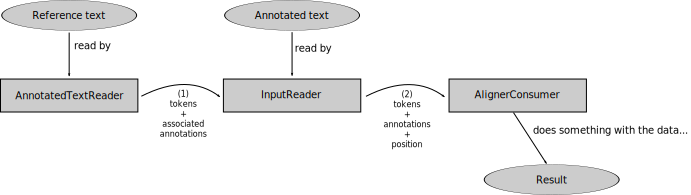
\includegraphics[width=\linewidth]{fig_principle_align.pdf}
\caption{\label{fig_principle_align} The \utilsPackname .align package: general principle}
\end{figure}


\begin{xenumerate}
\item An {\tt AnnotatedTextReader} object is responsible for reading the annotated text and tokenizing it incrementally. It transmits each token and possibly the annotation(s) related to this token to an {\tt InputReader} object.
\item An {\tt InputReader} object is responsible for reading the reference (source) text and tokenizing it incrementally (or managing to recover positions of tokens contained in the text in any way). When receiving data from the {\tt AnnotatedTextReader} object, it has to find the corresponding token in the original text and transmit the whole information to an {\tt AlignerConsumer} object.
\item Finally an {\tt AlignerConsumer} object receives the data and ``consumes'' it in some way: standard behaviours include writing the data into a file or in a String object, or writing it into the CAS in the UIMA case. There are different options about the form of the data it receives, depending on the need for all tokens or only annotated ones, positions of tokens, etc.
\end{xenumerate}

\subsubsection{Usage}

These three elements are provided as interfaces, except {\tt AnnotatedTextReader} which is an abstract class because it ``controls'' the whole process: it contains the main method {\tt align} which (normally) does not need to be overriden. This method simply calls the specific overriden methods in the other classes (see javadoc API for details). Several useful implemented classes are provided, among which:

\begin{xitemize}
\item {\tt SimpleTaggedTextReader} and {\tt SimpleTokenByLineReader} are two {\tt AnnotatedTextReader} objects. The former reads a text annotated with tags \verb+<mytag>...</mytag>+ (like in the above example). The latter reads a text annotated in the form of one token by line, followed by annotations, i.e. 

\verb+Peter  person+\\
\verb+(      -+\\
\verb+really -+\\
\verb+)      -+\\
\verb+loves  -+\\
\verb+Nutella       org+\\
\verb+.      -+

\item {\tt SimpleInputReader} and {\tt TokenIteratorInputReader} are two {\tt InputReader} objects. The former reads the source text from a {\tt Reader} object (file, String or stream), and the latter expects an already tokenized text provided using an {\tt Iterator} object.
\item {\tt TagAlignerWriterConsumer} and {\tt TagPositionConsumer} are {\tt AlignerConsumer} objects. The former writes the text together with its annotations to a {\tt Writer} object, while the latter is intended to deal with positions (this one has to be instanciated with a {\tt TagPositionConsumer.AnnotationReceiver} which is resposible to ``do something'' with the annotations and positions). Notice that contrary to the two previous classes the {\tt AlignerConsumer} object is generally totally overriden, because its behaviour is very specific.
\end {xitemize}


This modular approach permits to deal with different formats at any of the three levels in a similar way: for example it is possible to use any of the two {\tt InputReader} implemented classes with any of the two {\tt AnnotatedTextReader} implemented classes, and the same holds (more or less\footnote{Of course meaningless combinations do not work: reading ``token by line'' annotations from the annotated text as ``tags'' annotations in the consumer will surely fail.}) for {\tt AlignerConsumer} objects. This way a lot duplicate similar code is avoided, and the behaviour of all components using these classes is consistent (see \ref{part_good_practices}). Finally components using these objects only have to deal with their specific format issues, and do neither add duplicate code for the common parts of the process.




\section{Troubleshooting}
\label{partTroubleshooting}


\todo{1) regarder msg d'erreur complet (stack trace), 2) regarder log file 3) éventuellement changer le type de log et relancer ; distinguer erreurs à l'init et erreurs au process}



Here are listed several problems which can appear quite frequently with UIMA and/or the \uimaModule module, together with  their solution. Unfortunately it is not possible to propose an exhaustive list!

\subsubsection{UIMA general path problems}
\label{pathProblems}
{\bf Path problems} are very very frequent using UIMA, because of the descriptors system: where a classical Java program would simply include calls to some other packages/classes (and therefore missing classes would make the compilation fail with a clear statement of what is missing), with a UIMA program it is impossible to know whether something is missing at compilation time. Additionally:
\begin{xitemize}
\item there is no way to check that an XML descriptor is valid w.r.t the elements it refers to (other descriptors, Java classes);
\item the modular policy implies that there are a lot of such references;
\item the {\em ``by location''} references become wrong as soon as something changes in the filesystem (file or directory);
\item there can be confusions between references {\em ``by name''} and {\em ``by location''}.
\end{xitemize}

Therefore errors occur quite frequently, but the following recommendations may help:

\begin{xitemize}
\item Whenever possible, prefer {\bf import by name} rather than {\bf import by location}.  {\em import by name} means that the UIMA engine will look for the descriptor in the {\tt CLASSPATH}\footnote{or datapath (as far as I know this is the same in standard use). If you do not understand how Java works with {\tt CLASSPATH} (this is not specific to UIMA at all), please refer to some Java official documentation about that. In particular let me recall that the {\tt CLASSPATH} does not only contain Java classes, but can also contain any file, e.g. XML descriptors.}: this is a lot safer, because this way all the dependencies are contained in the same place (usually in a JAR archive) that you specify in your CLASSPATH.
\begin{xitemize}
\item common error with {\em import by name}: do not write the {\tt .xml} extension for the descriptors. UIMA engine will automatically look for the name plus its xml extension (and then will not find some {\tt mydesc.xml.xml} file!).
\item common error causing a descriptor missing in the {\tt CLASSPATH}: forgetting to copy the data directories (in particular {\tt desc} containing the descriptors) in the Java  output directory (usually {\tt bin}). See \ref{partCompile} for how to do so depending on the compilation method.
\item when using the UIMA CPE GUI tool (provided with UIMA) to create CPE descriptors, the imports are always written as {\em by location} absolute pathes. This is not convenient at all and causes frequent errors once you change anything in the filesystem. Either do no use this tool at all, or edit the descriptor by hand after creating it (see also \ref{partImportsCpeGui}).
\end{xitemize}
\item If ever using imports by location, do not use absolute pathes in locations but relative ones, otherwise the system is broken as soon as the project is moved elsewhere.
\item Have a clear strategy about where descriptors should be located, and what kind of import (reference) is used. When you perform changes in the {\tt CLASSPATH} folders structure, do not forget that it can impact descriptors.
\end{xitemize}


\subsubsection{Wrapped programs problems}

\begin{xitemize}
\item {\bf path problems}. if a CPE using \uimaModule complains at initialization step about not finding some file/directory/program, check: 
\begin{xenumerate}
\item that the external program called is installed on your system;
\item that it can be accessed by the way specified through the descriptor: the default structure is detailed in \ref{installExternalPrograms}. If the default does not meet your needs, you have to specify explicitly the location(s) in the descriptor (check the parameters descriptions to understand exactly what should be provided).
\end{xenumerate}
\end{xitemize}

\subsubsection{Yatea bugs}
\label{yateaBugs}

There are several bugs in Yatea 0.5\footnote{Yatea does not seem to be maintained anymore: I reported these bugs to Thierry Hamon (the author) and did not receive any answer. As far as I know the official CPAN module has not been modified for a few years.} (official current version). Below is a non exhaustive list together with some workarounds. Some of them are errors which are recovered by the Yatea AE provided in this package, but others are internal bugs: it is {\bf strongly recommended} to apply the changes for the latter\footnote{The script {\tt install-scripts/patch\_yatea.sh} can perform these changes for you.}.


\begin{itemize}
\item Symptom: in some cases the following fatal error stops the Yatea process:

\begin{verbatim}
Can't locate object method "getFather" via package "Lingua::YaTeA::RootNode" 
                  at [your-perl-modules-location]/Lingua/YaTeA/Node.pm line 1496.
\end{verbatim}

Cause: missing parentheses in two places (lines 1496 and 1528, same condition) in {\tt Node.pm} in the following condition (correction in red):
\begin{verbatim}
    if(
       (isa($node,'Lingua::YaTeA::InternalNode'))
&&
       ($node->getFather->getEdgeStatus($position) eq "HEAD")
&&
\end{verbatim}
{\color{red} \tt  (}
\begin{verbatim}
       (
        ($position eq "LEFT")
&&
        ($node->getRightEdge->searchLeftMostLeaf->getIndex < $to_insert)
        )
       ||
       (
        ($position eq "RIGHT")
&&
        ($node->getFather->getRightEdge->searchLeftMostLeaf->getIndex < $to_insert)
        )
\end{verbatim}
{\color{red} \tt  )}
\begin{verbatim}
       ) 
\end{verbatim}

This bug is corrected by {\tt install-scripts/patch\_yatea.sh} (you have to provide the path).

\item Symptom: in some cases the following fatal error stops the Yatea process:
\begin{verbatim}
Can't call method "getIndex" on an undefined value at 
                [your-perl-modules-location]/Lingua/YaTeA/Node.pm line 2099
\end{verbatim}

Cause: missing test in the following condition line 2097 in {\tt Node.pm} (correction in red):

\verb+if(+\textcolor{red}{\tt defined(\$new\_next) \&\& (}\verb+$new_next->getIndex > $index+{\tt\textcolor{red}{)})}

This bug is also corrected by {\tt install-scripts/patch\_yatea.sh} (you have to provide the path).

\item Symptom: when no term at all has been found, Yatea crashes with the following error:
\begin{verbatim}
Illegal division by zero at [your-perl-modules-location]/Lingua/YaTeA/Corpus.pm line 1299.
\end{verbatim}

Cause: no test for zero in division line 1299 in {\tt Corpus.pm} (correction in red):

\verb+$mean_occ=+{\tt\textcolor{red}{(scalar(keys \%\$term\_candidates\_h)>0)?(}}\verb+$total_occ/scalar keys %$term_candidates_h+{\tt\textcolor{red}{):'NaN'};}

This bug is also corrected by {\tt install-scripts/patch\_yatea.sh} (you have to provide the path).

\item Positioning strategy (more a particular feature than a bug): In Yatea output tokens are indexed according to their sentence number and position in this sentence. However the position index is also incremented by 1 at each token encountered, as if tokens were separatated by one space\footnote{Yatea is not provided with the actual corpus, its input is a TreeTagger file with one token by line.}. The Yatea AE (more precisely the {\tt YateaXMLOutputParser} class) deals with this indexing and recovers the original position in the text.

\item Errors in positioning: in some cases involving complex terms containing shorter terms, yatea will assign wrong position indexes. This happens where there are difference occurrences of the same term with different words orders. For instance, in a corpus containing both {\em "Pneumopathie lobaire inférieure droite infectieuse"}  and {\em "Pneumopathie infectieuse lobaire inférieure droite"} (and maybe other variants), Yatea is able to recognize that they both refer to the same term. But the Yatea output format does not permit different forms for a single term, so they are both assigned the same form (the first one): so far this is not an error (maybe a questionable design at worst); however it becomes bad when shorter terms are contained in these terms : probably because their position is computed by Yatea using the longer term from which they are extracted {\em possibly using the wrong form}, they can be assigned shifted position indexes. In the case of the long term, this is not too bad since it is still inside the terms bounds, but positions of the term itself (if it appears outside the context of the long term) are also wrong. The Yatea AE tries to recover the right position (and usually succeeds): see part \ref{yateaAE} for details.

\end{itemize}

\subsubsection{Miscellaneous}


\begin{xitemize}
\item {\bf Charset encoding}. Normally the AEs deal with most charset encoding issues, but errors can still happen in the following cases:
\begin{xitemize}
\item the input encoding is wrong or (more frequently) the input text actually contains invalid characters (w.r.t this encoding). Theoretically  in this case an I/O exception should be raised by the Collection Reader (i.e. at the beginning of the process). But for some unknown reason (?) Java seems not to report all errors, so the process continues until another conversion is needed and this is often when {\em writing} the data into another encoding that the error is reported. Such cases were encoutered but we do not have real solutions for that; nevertheless being aware of that behaviour may help the user fixing problems.  
\item the encoding expected by the program does not permit to represent some characters: this is an unavoidable restriction by the external program. If these characters can be ignored without serious consequences, the workaround consists in using the {\tt replaceCharacterCodingErrorReplacementValue} parameter (which is provided with all wrapper AEs in \uimaModule).
\end{xitemize}

See also \ref{partUimaEncoding}.
\item the {\bf UIMA Annotation visualizer}: if you do not see all annotations in the resulting files (or even no annotation at all), do not forget to check that you specify the right Type System descriptor to the visualizer (any type which is not defined in this TS will not be visible).
\item {\bf Java memory}: if the process stops with an exception related to lack of memory space, you need to specify more memory for the Java Virtual Machine, using the -Xms ans -Xmx options (see Java documentation). Be careful, when using a 32 bits architecture the JVM is usually limited to 1.5G to 3G.
\end{xitemize}
\label{partJavaMem}

\todo{pbm possible avec lia : -m 32, manque de mémoire}

\section{Future work}

\label{partFutureWork}

LINA components: \todo{\url{http://www.lina.univ-nantes.fr/-Composants-UIMA-.html}}



\begin{xitemize}
\item Continue to test the platform in various cases, possibly correct/improve code.
\item Develop new / integrate existing annotators. There are different ideas that LIPN may study:
\begin{xitemize}
\item A term tagger, because it is a very useful component for LIPN,
\item A syntaxic parser, which would be useful of course but would also have another interest: it is indeed interesting to create/test concurrent annotations in a context where there are possibly different nested structures (due to syntactic ambiguities),
\item A customizable tokenizer, based on applying some rules defined by the user.
\end{xitemize}
\end{xitemize}

\subsubsection{LIA {\tt bin/lia\_nomb2alpha} Numbers converter}

Among LIA programs there is number converter named {\tt lia\_nomb2alpha}, which converts (digits) numbers into their expanded (letters) form. This program is supposed to be called after tokenizing the input text (as tokens and sentences), and before calling the POS tagger {\tt bin/lia\_tagg}. In particular it is used in the LIA NE named entities recognizer, and probably this NER performs better if this preprocessing step has been applied. It seems to work only for French, because there is no English corresponding resource. Here is an example:

\begin{verbatim}
echo "Parmi les 2397 personnes présentes le 25 avril 2008, 12 possèdent plus de 41,53 $." |
 $LIA_TAGG/bin/lia_tokenize $LIA_TAGG/data/lex80k.fr.tab |
 $LIA_TAGG/bin/lia_sentence $LIA_TAGG/data/list_chif_virgule.fr.tab |
 $LIA_TAGG/bin/lia_nett_capital $LIA_TAGG/data/lex80k.fr.tab |
 $LIA_TAGG/bin/lia_nomb2alpha $LIA_TAGG/data/list_chif_virgule.fr.tab
\end{verbatim}

This command output is:

\begin{verbatim}
<s>
parmi les deux mille trois cent quatre vingt dix sept personnes
présentes le vingt cinq avril deux mille huit , douze possèdent
plus de quarante et un virgule cinquante trois dollars . </s>
\end{verbatim}

Notice that this text is tokenized as follows (obtained by running the same command without the last line):

\begin{verbatim}
<s>
parmi les 2397 personnes présentes le 25 avril 2008 , 12 possèdent
plus de 41 , 53 $ .
</s>
\end{verbatim}

Thus as one can see this tools has the particularity not only to {\em transform} the input text (contrary to simply {\em add} some information), but also to transform a given token into several tokens. In the next steps (e.g. POS tagging) these tokens will be considered exactly as original tokens. There are two issues with this behaviour:

\begin{itemize}
\item The first issue is: how is it possible to represent such a transformation in the CAS ? This question is not trivial, but there are approaches to solve it. In particular we could use our {\em concurrent annotation} mechanism (see \ref{partConcurrentAnnot}: for example it is possible to use the {\tt Interpretation} type to build an annotation containing the annotations concerning each such special element (typically it would contain a list of {\tt Token} types, and probably {\tt PartOfSpeech} types etc. later). Moreover that would be consistent with the general idea of concurrent annotation: seeing numbers in their expanded form is another point of view on these tokens, and it is a reasonably useful information to keep.
\item The second issue is a simple technical problem: it is necessary for each UIMA wrapper annotator engine to be able to interpret the external program output, in particular to be able to locate exactly any information it receives. This is usually done using the alignment tools (see \ref{partAlign}) which compare the source input text to the annotated text, and for each annotated token return its position in the source text to know where the added information should go. Considering several tokens at once is not a problem, as soon as it is always possible to know where the annotation starts and ends. Unfortunately this is where things go wrong here, because there can be any number of consecutive ``old'' tokens transformed in any number of ``new'' tokens. Therefore there is no way to know where the first token ends and the second begins, like in the example: without knowing exactly how the program works, it is impossible to tell which new tokens concern ``{\tt 41}'', which ones concern ``{\tt ,}'', etc. 
\end{itemize}

One can notice that the problem would be solved if the program output had follow the original tokenization in any way, e.g. by providing the set of (new) tokens corresponding to a given (old) token on the same line. This is not the case, even if the tokens are provided one per line (to check call {\tt \$LIA\_TAGG/bin/unmotparligne} before {\tt bin/lia\_nomb2alpha} in the previous example).

This is why it is (at least currently) impossible  to integrate LIA {\tt bin/lia\_nomb2alpha} to the \softName platform.


\section{Glossary}

For UIMA terms and acronyms, please refer to UIMA official documentation. In particular, a convenient glossary is proposed in the ``Overview and Setup'' part\footnote{\url{http://uima.apache.org/downloads/releaseDocs/2.3.0-incubating/docs/html/overview_and_setup/overview_and_setup.html\#ugr.glossary}}.

\begin{xitemize}
\item \glossEntry{Alignment}{In \softName, refers to the re-alignment process needed when trying to integrate the annotations added by some external program into the source text. It is then necessary to find the exact corresponding part between the annotated text and the original one. The {\tt \utilsPackname .align} package is provided to do this task, see \ref{part_align_package}}
\item \glossEntry{CAS (Common Analysis Structure)}{The main UIMA data structure containing the document data, the Type System and the annotations. See UIMA documentation.}
\item{{\tt CLASSPATH} }{ The standard environment variable which contains the locations where Java looks for classes (and any other files). Since this mechanism is very important to understand how descriptors and classes work together in UIMA, refer to the Java official documentation in case you are not confortable with it.}
\item \glossEntry{Concurrency}{Can refer to two very different points that should not be confused: the usual {\em ``time'' concurrency} refers to using different threads to process different tasks at the same time (see Threads/Concurrency). Whereas {\em annotations concurrency} (concurrent annotations) is about different sets of annotations existing in the same environment (see Concurrent annotations).}
\item \glossEntry{Concurrent annotations}{Refers to the case where different sets (or series) of annotations which are independent are used in the same environment, typically the same CAS. In general these series have more or less the same ``role'' (e.g. different tokenizations of a text), this is why it may be an issue for an annotator not to confuse between the different series (see \ref{partConcurrentAnnot}).}
\item \glossEntry{CPE}{Collection Processing Engine. From ``UIMA Overview and Setup'': {\em Performs Collection Processing through the combination of a Collection Reader, zero or more Analysis Engines, and zero or more CAS Consumers. The Collection Processing Manager (CPM) manages the execution of the engine. The CPE also refers to the XML specification of the Collection Processing engine. The CPM reads a CPE specification and instantiates a CPE instance from it, and runs it.} 
}
\item \glossEntry{External program}{A non-Java program called by a wrapper annotator using a system call (an equivalent to {\tt Runtime.getRuntime().exec(String)}). A package is devoted to running such a program, see \ref{partExternalProgram}.}
\item \glossEntry{{\tt ReaderConsumer} (interface)}{ An object implementing this interface is able to read the content of a {\tt Reader} object when its {\tt consumeReader} method is called. Used to read an external program output on the fly, see \ref{ReaderConsumerWriterFeeder}.}
\item \glossEntry{Threads/Concurrency}{Running different threads to process different tasks at the same time. This is an issue if they share the same CAS (see \ref{partThreadsConcurrency})}
\item \glossEntry{Wrapper}{A component whose main task is actually proceded by some sub-component which was not intended to be used in this context. Thus this sub-component has a ``black box'' behaviour, since there can be no communication between it and the main process. See \ref{partWrapper}.}
\item \glossEntry{{\tt WriterFeeder} (interface)}{ An object implementing this interface is able to write some data to a {\tt Writer} object when its {\tt feedWriter} method is called. Used to write the external program input on the fly, see \ref{ReaderConsumerWriterFeeder}.}
\end{xitemize}


\bibliographystyle{plain}
\bibliography{TAL_BIB}


\end{document}
